\documentclass[12pt,spanish,Letterpaper,openany]{book}
\usepackage{lmodern}
\usepackage{setspace}
\setstretch{0.85}
\usepackage{amssymb,amsmath}
\usepackage{ifxetex,ifluatex}
\usepackage{fixltx2e} % provides \textsubscript
\ifnum 0\ifxetex 1\fi\ifluatex 1\fi=0 % if pdftex
  \usepackage[T1]{fontenc}
  \usepackage[utf8]{inputenc}
\else % if luatex or xelatex
  \ifxetex
    \usepackage{mathspec}
  \else
    \usepackage{fontspec}
  \fi
  \defaultfontfeatures{Ligatures=TeX,Scale=MatchLowercase}
    \setmainfont[Scale=1.0, HyphenChar=None]{Corbel}
    \setsansfont[]{Corbel}
    \setmonofont[Mapping=tex-ansi]{Corbel}
\fi

\makeatletter
\renewcommand\mainmatter{\clearpage\@mainmattertrue\pagenumbering{arabic}}
\renewcommand\frontmatter{\clearpage\@mainmatterfalse\pagenumbering{arabic}}
\renewcommand\backmatter{\clearpage\@mainmatterfalse}
\makeatother

%\usepackage{etoolbox}
%\makeatletter
%\patchcmd{\@smemmain}{\cleardoublepage}{\clearpage}{}{}
%\patchcmd{\@smemmain}{\cleardoublepage}{\clearpage}{}{}
%\patchcmd{\@smemfront}{\cleardoublepage}{\clearpage}{}{}
%\patchcmd{\@smemfront}{\cleardoublepage}{\clearpage}{}{}
%\makeatother

\setlength{\parindent}{0em}

\usepackage{graphicx}
\usepackage{booktabs}
\usepackage{multicol}
\usepackage{doc}
\usepackage{float}
\usepackage{tcolorbox} 
\usepackage{lipsum}
\usepackage{tikz}
\usepackage{nonfloat}

\usepackage{pdfpages}

\usepackage[
contents={},
opacity=1,
scale=1.5,
color=blue!90
]{background}
\usepackage{lipsum}
\usepackage{ifthen}

\usepackage{xcolor}
\usepackage[pagestyles]{titlesec}

\renewpagestyle{plain}[\normalsize\sffamily\bfseries\slshape]{
  \setfoot{}{\color{white}{\thepage}}{}}

\newpagestyle{myps}[\normalsize\sffamily\bfseries\slshape]{
  \setfoot{}{\color{white}{\thepage}}{}}
  
\pagestyle{myps}


\usepackage{framed}
\definecolor{colorlinetitle}{HTML}{6a78de}%{cfb23e}%
\definecolor{textlinetitle}{HTML}{001077}%{25408F}%{243F8E}%
\definecolor{fondo}{HTML}{f2d37e}%
\definecolor{newfondo}{HTML}{d6b72d}%
\colorlet{shadecolor}{fondo!81!}


% use upquote if available, for straight quotes in verbatim environments
\IfFileExists{upquote.sty}{\usepackage{upquote}}{}
% use microtype if available
\IfFileExists{microtype.sty}{%
\usepackage{microtype}
\UseMicrotypeSet[protrusion]{basicmath} % disable protrusion for tt fonts
}{}
\usepackage[inner=12.7mm,outer=12.7mm,top=25mm,bottom=21.0mm]{geometry}
\usepackage{hyperref}
\hypersetup{unicode=true,
            pdftitle={Revista de la Unidad de Prácticas de Ingeniería y EPS},
            pdfauthor={Unidad de Prácticas de Ingeniería y EPS},
            pdfborder={0 0 0},
            breaklinks=true}
\urlstyle{same}  % don't use monospace font for urls
\ifnum 0\ifxetex 1\fi\ifluatex 1\fi=0 % if pdftex
  \usepackage[shorthands=off,main=spanish]{babel}
\else
  \usepackage{polyglossia}
  \setmainlanguage[]{spanish}
\fi
\usepackage{natbib}
\bibliographystyle{apalike}
\usepackage{longtable,booktabs}
\IfFileExists{parskip.sty}{%
\usepackage{parskip}
}{% else
\setlength{\parindent}{0pt}
\setlength{\parskip}{6pt plus 2pt minus 1pt}
}
\setlength{\emergencystretch}{3em}  % prevent overfull lines
\providecommand{\tightlist}{%
  \setlength{\itemsep}{0pt}\setlength{\parskip}{0pt}}
\setcounter{secnumdepth}{5}
% Redefines (sub)paragraphs to behave more like sections
\ifx\paragraph\undefined\else
\let\oldparagraph\paragraph
\renewcommand{\paragraph}[1]{\oldparagraph{#1}\mbox{}}
\fi
\ifx\subparagraph\undefined\else
\let\oldsubparagraph\subparagraph
\renewcommand{\subparagraph}[1]{\oldsubparagraph{#1}\mbox{}}
\fi

%%% Use protect on footnotes to avoid problems with footnotes in titles
\let\rmarkdownfootnote\footnote%
\def\footnote{\protect\rmarkdownfootnote}


  \title{Revista de la Unidad de Prácticas de Ingeniería y EPS}
    \author{Unidad de Prácticas de Ingeniería y EPS}
      \date{2021-10-19}

% no title page
\AtBeginDocument{\let\maketitle\relax}

\usepackage{caption}
\captionsetup{%
labelsep=colon,%
font={footnotesize},%
aboveskip=0.5\baselineskip,%
belowskip=0\baselineskip,% deve essere 0 perché regolo lo spazio dal testo con \intextsep
}%


\usepackage{booktabs}
\usepackage{longtable}

\usepackage{indentfirst}
\setlength{\parindent}{1em}
\usepackage{enumitem}
\setlist[itemize]{labelindent = \parindent, leftmargin=*}

%\usepackage{framed,color}
%\definecolor{shadecolor}{RGB}{248,248,248}

\renewcommand{\textfraction}{0.05}
\renewcommand{\topfraction}{0.8}
\renewcommand{\bottomfraction}{0.8}
\renewcommand{\floatpagefraction}{0.75}

\renewcommand{\chaptername}{Artículo}
\addto\captionsspanish{\renewcommand{\chaptername}{Artículo}}
\addto\captionsspanish{\renewcommand{\contentsname}{Índice general}}


\frenchspacing
\tolerance=5000
\multicoltolerance=3000 

\raggedbottom
\raggedcolumns

\setlength{\columnsep}{1em}
%We want a rule between columns.
%\setlength\columnseprule{.4pt}

%Tambien queremos asegurarnos de que un nuevo entorno multicols 
%encuentre suficiente espacio en la parte inferior de la pagina.
\setlength\premulticols{6\baselineskip}

%Al equilibrar columnas, ignoramos las soluciones que son 
%demasiado malas. Ademas, si la ultima columna es demasiado mala, 
%la tipeamos sin estirar.
\setcounter{columnbadness}{7000}
\setcounter{finalcolumnbadness}{7000}

\newcommand{\prefacetitlecommand}%
{\titleformat{\chapter}[display]%
{\bfseries\large\color{colorlinetitle}}%
{\relax}%
{0ex}%
{{\titlerule[1.2pt]}\filright\color{textlinetitle}}[\color{colorlinetitle}\vspace{0.5ex}{\titlerule[1.2pt]}]%
}


\newcommand{\articletitlecommand}%
{\titleformat{\chapter}[display]%
{\bfseries\large\color{colorlinetitle}}%
{\relax}%
{0ex}%
{{\titlerule[1.2pt]}\filright\color{textlinetitle}}[\color{colorlinetitle}\vspace{0.5ex}{\titlerule[1.2pt]}]%
}



\newcommand{\sectionCenter}%
{\titleformat{\section}[block]%
{\bfseries\large\color{textlinetitle}\filcenter}%
{\relax}%
{0ex}%
{\empty}%
}


\newcommand{\sectionRight}%
{\titleformat{\section}[block]%
{\bfseries\large\color{textlinetitle}}%
{\relax}%
{0ex}%
{\empty}%
}


\newcommand{\subsectionRight}%
{\titleformat{\subsection}[block]%
{\bfseries\normalsize\color{textlinetitle}}%
{\relax}%
{0ex}%
{\empty}%
}

\usepackage{titletoc}
\titlecontents{chapter}[3em]
{\vspace{5mm}}
{\normalsize\contentslabel[\color{textlinetitle}\thecontentslabel]{2em}\color{black}\itshape\normalsize}
{\color{black}\itshape\normalsize}
{\color{colorlinetitle}\titlerule*[.3pc]{.}\color{black}\contentspage}

\newcommand{\tcolorboxcommand}{\begin{tcolorbox}[sharp corners=uphill, colback=newfondo, colframe=newfondo, arc=6mm, boxrule=0mm, boxsep=0mm]}

\newcommand{\photocommand}[2]{%
\fcolorbox[HTML]{DCEEA7}{DCEEA7}{%
\begin{minipage}{95.19mm}%
	\hspace{1mm}%
	\begin{minipage}{22.49mm}%
		\vspace{1mm}%
		\includegraphics[width=22.49mm, height=31.96mm]{#1}%
		\vspace{1mm}%
	\end{minipage}%
	\hspace{2.4mm}%
	\begin{minipage}{68.80mm}%
		#2
	\end{minipage}%
	\hspace{0.5mm}%
\end{minipage}%
}%
}

\definecolor{fondobiography}{HTML}{DCEEA7}

\NewDocumentEnvironment{photobiography}{m O{}}%
{%
\begin{tcolorbox}[colback=fondobiography, colframe=fondobiography, width=97.19mm, boxsep=-2mm, arc=0mm]
\begin{minipage}{95.19mm}%
	%\hspace{1mm}%
	\begin{minipage}{22.49mm}%
		\vspace{2mm}%
		\includegraphics[width=22.49mm, height=31.96mm]{#1}%
		\vspace{2mm}%
	\end{minipage}%
	\hspace{2.4mm}%
	\begin{minipage}{68.80mm}%
	#2%
}%
{%
	\end{minipage}%
	%\hspace{0.5mm}%
\end{minipage}%
\end{tcolorbox}
}


\newcommand{\spacetext}{\vspace{8.1mm}}
\newcommand{\minimalspacetext}{\vspace{1mm}}
\newcommand{\spaceelevenmilis}{\vspace{11mm}}
\newcommand{\spacetenmilis}{\vspace{10mm}}
\newcommand{\spaceninemilis}{\vspace{9mm}}
\newcommand{\spaceeightmilis}{\vspace{8mm}}
\newcommand{\spacesevenmilis}{\vspace{7mm}}
\newcommand{\spacesixmilis}{\vspace{6mm}}
\newcommand{\spacefivemilis}{\vspace{5mm}}
\newcommand{\spacefourmilis}{\vspace{4mm}}
\newcommand{\spacethreemilis}{\vspace{3mm}}
\newcommand{\spacetwomilis}{\vspace{2mm}}
\newcommand{\spaceinitialeditorialcontenido}{\vspace{8.1mm}}
\newcommand{\spaceoneminus}{\vspace{-1mm}}
\newcommand{\spacetwominus}{\vspace{-2mm}}
\newcommand{\spacefourminus}{\vspace{-4mm}}
\newcommand{\hideFromPandoc}[1]{#1}
\hideFromPandoc{ \let\Begin\begin \let\End\end }
\newcommand{\minipagepartone}{\begin{minipage}[c]{3cm}}
\newcommand{\minipagetwocolumn}{\noindent\begin{minipage}[c]{\columnwidth}}
\newcommand{\minipageparttwo}{\end{minipage}\begin{minipage}[c]{12cm}}
\newcommand{\minipageparttwochapter}{\end{minipage}\begin{minipage}[c]{15cm}}
\newcommand{\minipageendpart}{\end{minipage}}
\newcommand{\firstparteditorial}{\begin{longtable}[]{@{}ll@{}}\endhead\begin{minipage}[t]{0.47\columnwidth}\raggedright}
\newcommand{\firstparttwoeditorial}{\begin{longtable}[l]{@{}ll@{}}\endhead\begin{minipage}[t]{0.47\columnwidth}\raggedright}
\newcommand{\midleparteditorial}{\end{minipage} & \begin{minipage}[t]{0.47\columnwidth}\raggedright}
\newcommand{\lastparteditorial}{\end{minipage}\end{longtable}}

\newcommand{\HRule}{\begin{center}\rule{0.5\linewidth}{0.2mm}\end{center}}

\begin{document}
\maketitle

% \pagestyle{plain}

\includepdf{images/cover.pdf}

\AddEverypageHook{%
\ifthenelse{\value{page}<32}%
{\ifthenelse{\isodd{\value{page}}}%
  	{\backgroundsetup{scale=1, color=black, opacity=1, angle=0, contents={
\includegraphics[width=\paperwidth,height=\paperheight]{latex/background_numberimpar.pdf}}}}%
  	{\backgroundsetup{scale=1, color=black, opacity=1, angle=0, contents={
\includegraphics[width=\paperwidth,height=\paperheight]{latex/background_numberpar.pdf}}}}%
}{}%
\BgMaterial}

%%%%%%{
%%%%%%\setcounter{tocdepth}{0}
%%%\tableofcontents
%%%}
%%%%%%%%%%%%\listoffigures
%%%
\prefacetitlecommand

\titlespacing*{\chapter} {0pt}{0pt}{2pt}

\addtocontents{toc}{\vspace{3mm}~\hfill\color{textlinetitle}\textbf{Pág.}\vspace{3mm}\par}

\hypertarget{index}{%
\chapter*{Editorial}\label{index}}
\addcontentsline{toc}{chapter}{Editorial}

\begin {flushright}

\emph{Tan solo por la educación puede el hombre llegar a ser hombre.}

\emph{El hombre no es más que lo que la educación hace de él (Emmanuel Kant)}

\end {flushright}

\begin{center}
\includegraphics[width=0.2\linewidth]{images/editorial} \end{center}

\begin {center}

\textbf{Responsabilidad, conocimiento y experiencia en el egresado universitario}

\end {center}

El éxito para concluir una carrera universitaria radica en la voluntad y actitud del estudiante. Su deseo de ser profesional triunfador debe ser una manifestación auténtica en todas las actividades que impliquen conocimiento y experiencia en su formación académica. El éxito estará definido desde el momento en que selecciona una carrera, porque esta es la consecuencia de aspiraciones e intereses atesorados desde su niñez, los cuales hará realidad en las aulas universitarias. La responsabilidad y compromiso son valores que añadirá cuando se desenvuelva profesionalmente. Esta será la consolidación de su éxito profesional. En el ámbito laboral o empresarial desarrollará sus aptitudes, habilidades y liderazgo; esto evidenciará la efectividad y fortalecimiento de un aprendizaje significativo a nivel superior.

Ampliar el perímetro del conocimiento y la experiencia permitirá al egresado universitario ser parte de una dinámica social cambiante en un medio en el cual la tecnología es parte del ejercicio diario del ser humano. Allí podrá advertirse la prevalencia de muchos elementos vinculados con su formación.

¡Qué nivel de madurez puede observarse en el estudiante próximo a graduarse! El informe de EPS o la elaboración de su tesis serán la feliz evidencia de haber concluido sus estudios exitosamente. La validez y cientificidad de su contenido serán la consecuencia del aprovechamiento académico en las aulas. En relación con este valioso documento, vale la pena sugerir al estudiante de la Facultad de Ingeniería que utilice el instructivo y formato diseñado por la Unidad de Lingüística, y aplique el normativo específico ya sea de pregrado, pre-post y posgrado; el mismo constituye la guía ineludible para facilitar su elaboración. De esta manera se acelerará el proceso y presentará un trabajo de calidad.

En el desenvolvimiento diario del nuevo profesional perdurará el recuerdo de sus años estudiantiles e incidirá el ejemplo de sus docentes, porque fueron capaces de transformar sus vidas y convertirlos en personas de éxito. Recordemos que:

\begin{center}
En el aula se construye con el docente por guía, la ciencia y tecnología. El aprendizaje fluye si el educando se instruye con lo que aplicar prefiere.
El conocimiento adquiere si se orienta con amor, cuando cumple el profesor con lo que el medio requiere.


\end{center}

\begin {center}

\textbf{Aura Mayorga Salguero}

\end {center}

\medskip

\HRule

\medskip

\newpage

\hypertarget{directorio}{%
\chapter*{Directorio}\label{directorio}}
\addcontentsline{toc}{chapter}{Directorio}

\spacetwomilis

\begin{center}
\includegraphics{images/201901-logo} \end{center}
\spacetwominus

\sectionCenter

\hypertarget{nuxf3mina-de-junta-directiva}{%
\section*{Nómina de Junta Directiva}\label{nuxf3mina-de-junta-directiva}}
\addcontentsline{toc}{section}{Nómina de Junta Directiva}

\begin{longtable}[]{@{}ll@{}}
\endhead
\begin{minipage}[t]{0.239\columnwidth}\raggedright
DECANA\strut
\end{minipage} & \begin{minipage}[t]{0.35\columnwidth}\raggedright
Inga. Aurelia Anabela Cordova Estrada\strut
\end{minipage}\tabularnewline
\begin{minipage}[t]{0.239\columnwidth}\raggedright
VOCAL I\strut
\end{minipage} & \begin{minipage}[t]{0.35\columnwidth}\raggedright
Ing. José Francisco Gómez Rivera\strut
\end{minipage}\tabularnewline
\begin{minipage}[t]{0.239\columnwidth}\raggedright
VOCAL II\strut
\end{minipage} & \begin{minipage}[t]{0.35\columnwidth}\raggedright
Ing. Mario Renato Escobedo Martínez\strut
\end{minipage}\tabularnewline
\begin{minipage}[t]{0.239\columnwidth}\raggedright
VOCAL III\strut
\end{minipage} & \begin{minipage}[t]{0.35\columnwidth}\raggedright
Ing. José Milton de León Bran\strut
\end{minipage}\tabularnewline
\begin{minipage}[t]{0.239\columnwidth}\raggedright
VOCAL IV\strut
\end{minipage} & \begin{minipage}[t]{0.35\columnwidth}\raggedright
Br. Kevin Armando Cruz Lorente\strut
\end{minipage}\tabularnewline
\begin{minipage}[t]{0.239\columnwidth}\raggedright
VOCAL V\strut
\end{minipage} & \begin{minipage}[t]{0.35\columnwidth}\raggedright
Br. Fernando José Paz González\strut
\end{minipage}\tabularnewline
\begin{minipage}[t]{0.239\columnwidth}\raggedright
SECRETARIO\strut
\end{minipage} & \begin{minipage}[t]{0.35\columnwidth}\raggedright
Ing. Hugo Humberto Rivera Pérez\strut
\end{minipage}\tabularnewline
\end{longtable}

\spacetwominus

\sectionRight
\subsectionRight

\begin{longtable}[]{@{}ll@{}}\endhead\begin{minipage}[t]{0.47\columnwidth}\raggedright

\hypertarget{directorio-1}{%
\section*{Directorio}\label{directorio-1}}
\addcontentsline{toc}{section}{Directorio}

\textbf{Ingeniero Oscar Argueta Hernández}\\
Dirección de Prácticas de Ingeniería y EPS
\spacethreemilis

\hypertarget{editor-en-jefe}{%
\subsection*{Editor en Jefe}\label{editor-en-jefe}}
\addcontentsline{toc}{subsection}{Editor en Jefe}

\textbf{Ingeniera Floriza Avila Pesquera de Medinilla}\\
Coordinadora del Área de Tecnología\\
Unidad de Prácticas de Ingeniería
\spacethreemilis

\hypertarget{coeditores}{%
\subsection*{Coeditores}\label{coeditores}}
\addcontentsline{toc}{subsection}{Coeditores}

\textbf{Ingeniero Juan Merck Cos}\\
Asesor Supervisor del Área de Ingeniería Civil\\
Unidad de Prácticas de Ingeniería
\spacethreemilis

\textbf{Ingeniero Silvio José Rodríguez Serrano}\\
Asesor Supervisor del Área de Ingeniería Civil\\
Unidad de Prácticas de Ingeniería
\spacethreemilis

\textbf{Ingeniera Sigrid Alitza Calderón de De Léon}\\
Asesor Supervisor del Área de Ingeniería Industrial y Mecánica Industrial\\
Unidad de Prácticas de Ingeniería

\end{minipage} & \begin{minipage}[t]{0.47\columnwidth}\raggedright

\hypertarget{consejo-editorial}{%
\section*{Consejo Editorial}\label{consejo-editorial}}
\addcontentsline{toc}{section}{Consejo Editorial}

\textbf{Ingeniero Oscar Argueta Hernández}\\
Asesor Supervisor del Área de Ingeniería Civil\\
Unidad de Prácticas de Ingeniería
\spacethreemilis

\textbf{Ingeniera Floriza Avila Pesquera de Medinilla}\\
Asesor Supervisor del Área de Ingeniería de Ciencias y Sistemas\\
Unidad de Prácticas de Ingeniería
\spacethreemilis

\textbf{Ingeniero Juan Merck Cos}\\
Asesor Supervisor del Área de Ingeniería Civil\\
Unidad de Prácticas de Ingeniería
\spacethreemilis

\textbf{Ingeniero Carlos Anibal Chicojay Coloma}\\
Asesor Supervisor del Área de Ingeniería Mecánica\\
Unidad de Prácticas de Ingeniería
\spacethreemilis

\textbf{Ingeniera Sigrid Alitza Calderón de De Léon}\\
Asesor Supervisor del Área de Ingeniería Industrial y Mecánica Industrial\\
Unidad de Prácticas de Ingeniería
\spacethreemilis

\textbf{Ingeniera Norma Ileana Sarmiento de Serrano}\\
Asesor Supervisor del Área de Ingeniería Industrial y Mecánica Industrial\\
Unidad de Prácticas de Ingeniería

\end{minipage}\end{longtable}
\begin{longtable}[l]{@{}ll@{}}\endhead\begin{minipage}[t]{0.47\columnwidth}\raggedright

\hypertarget{comituxe9-editorial}{%
\section*{Comité Editorial}\label{comituxe9-editorial}}
\addcontentsline{toc}{section}{Comité Editorial}

\textbf{Ingeniero Oscar Argueta Hernández}\\
Asesor Supervisor del Área de Ingeniería Civil\\
Unidad de Prácticas de Ingeniería
\spacefourmilis

\textbf{Ingeniera Floriza Avila Pesquera de Medinilla}\\
Asesor Supervisor del Área de Ingeniería de Ciencias y Sistemas\\
Unidad de Prácticas de Ingeniería
\spacefourmilis

\textbf{Ingeniero Juan Merck Cos}\\
Asesor Supervisor del Área de Ingeniería Civil\\
Unidad de Prácticas de Ingeniería
\spacefourmilis

\textbf{Ingeniero Carlos Anibal Chicojay Coloma}\\
Asesor Supervisor del Área de Ingeniería Mecánica
Unidad de Prácticas de Ingeniería
\spacefourmilis

\textbf{Ingeniera Sigrid Alitza Calderón de De Léon}\\
Asesor Supervisor del Área de Ingeniería Industrial y Mecánica Industrial\\
Unidad de Prácticas de Ingeniería
\spacefourmilis

\textbf{Ingeniera Norma Ileana Sarmiento de Serrano}\\
Asesor Supervisor del Área de Ingeniería Industrial y Mecánica Industrial\\
Unidad de Prácticas de Ingeniería
\spacefourmilis

\textbf{Ingeniero Silvio José Rodríguez Serrano}\\
Asesor Supervisor del Área de Ingeniería Civil\\
Unidad de Prácticas de Ingeniería
\spacefourmilis

\textbf{Licenciada Aura Mayorga Salguero}\\
Revisión y estilo
\spacefourmilis

\textbf{Jenny Sharai Montenegro Contreras}\\
Redacción, diseño y diagramación
\spacefourmilis

\end{minipage}\end{longtable}

\setcounter{tocdepth}{0}
\tableofcontents

\articletitlecommand

\titlespacing*{\chapter} {0pt}{-20pt}{4pt}

\setstretch{0.91}

\hypertarget{unidadeps}{%
\chapter[Unidad de Prácticas de Ingeniería y Ejercicio Profesional Supervisado ]{\texorpdfstring{Unidad de Prácticas de Ingeniería y Ejercicio Profesional Supervisado \footnote{\url{http://eps.ingenieria.usac.edu.gt/}}}{Unidad de Prácticas de Ingeniería y Ejercicio Profesional Supervisado }}\label{unidadeps}}

\begin{center}
\includegraphics[width=1\linewidth]{images/eps} \end{center}
\smallskip

\begin {multicols}{2}

\hypertarget{introducciuxf3n}{%
\section*{Introducción}\label{introducciuxf3n}}
\addcontentsline{toc}{section}{Introducción}

La Unidad de Ejercicio Profesional Supervisado (EPS) depende directamente de la Decanatura de la Facultad de Ingeniería, es la Unidad oficial encargada de administrar y darle seguimiento a los programas de Ejercicio Profesional Supervisado de Graduación de la Facultad de Ingeniería, en coordinación con las diferentes escuelas.

La Universidad de San Carlos de Guatemala, a través de sus diferentes programas de extensión, permite una vinculación con la sociedad guatemalteca, contribuyendo a la solución de la problemática nacional y al mejoramiento de la calidad de vida de sus habitantes.

Dentro de estos programas, la Facultad de Ingeniería cuenta con el Ejercicio Profesional Super-
visado (E.P.S.), trabajando en coordinación con diferentes instituciones públicas y privadas como: Municipalidades, Ministerios, Cooperativas, Orga-
nismos No Gubernamentales, Ingenios Azucareros, Fundaciones, Hospitales, Dependencias de la Univer-
sidad de San Carlos de Guatemala, entre otros.

El EPS incluye actividades académicas de servicio técnico-profesional universitario de investigación y docencia-aprendizaje que los estudiantes con cierre de pénsum de estudios realizan en el medio real del país, para resolver problemas relativos a su profesión.

Por medio de esta práctica, los estudiantes próximos a graduarse, ejercitan su profesión, apoyados y orientados por los asesores-supervisores docentes, para formar profesionalmente a los estudiantes y prestar servicios a la sociedad.

\hypertarget{misiuxf3n}{%
\section*{Misión}\label{misiuxf3n}}
\addcontentsline{toc}{section}{Misión}

Complementar y fortalecer la formación académica de los estudiantes de las distintas carreras de la Facultad de Ingeniería de la Universidad de San Carlos de Guatemala, a través de la realización de las Prácticas de Ingeniería y el Ejercicio Profesional Supervisado, aplicando los conocimientos, habilidades (destrezas) y criterios adquiridos durante la formación académica a problemas reales a los que se enfrentará, adquiriendo conciencia de la realidad nacional, formándose como un futuro profesional comprome-
tido con el desarrollo del país, en su entorno social y ecológico.

\hypertarget{visiuxf3n}{%
\section*{Visión}\label{visiuxf3n}}
\addcontentsline{toc}{section}{Visión}

Ser la dependencia de la Facultad de Ingeniería que complemente la formación profesional de los estudiantes de las diferentes especialidades de la Ingeniería, para que integren los conocimientos, habilidades (destrezas) y criterios adquiridos durante su carrera, con el fin de formar profesionales con principios éticos y excelencia académica comprome-
tidos a integrarse en los diversos sectores de la sociedad.

\hypertarget{objetivos}{%
\section*{Objetivos}\label{objetivos}}
\addcontentsline{toc}{section}{Objetivos}

\hypertarget{general}{%
\subsection*{General}\label{general}}
\addcontentsline{toc}{subsection}{General}

Sistematizar y enriquecer los conocimientos del estudiante al interpretar objetivamente la realidad nacional, mediante la confrontación cotidiana de la teoría con la práctica.

\hypertarget{especuxedficos}{%
\subsection*{Específicos}\label{especuxedficos}}
\addcontentsline{toc}{subsection}{Específicos}

\begin{itemize}
\item
  Participar en las diferentes comunidades, institu-
  ciones y empresas asignadas como centros de Prácticas a través del Ejercicio Profesional Supervisado de la Facultad de Ingeniería de la Universidad de San Carlos de Guatemala; dándole prioridad a aquellas que realicen actividades no lucrativas o que realicen funciones de interés social.
\item
  Generar un proceso de participación y autoges-
  tión en las comunidades, instituciones y empresas, a fin de promover o fortalecer su organización como instrumento para el impulso del desarrollo social permanentemente y sostenible.
\item
  Fortalecer la formación profesional de los futuros egresados, mediante un trabajo supervisado que integre y aplique los conocimientos adquiridos durante la carrera.
\item
  Contribuir a que los estudiantes desarrollen la capacidad de análisis e interpretación de la problemática nacional.
\item
  Promover las actividades de docencia, investi-
  gación y extensión universitaria con participación interinstitucional en el ámbito nacional.
\end{itemize}

\hypertarget{organigrama}{%
\section*{Organigrama}\label{organigrama}}
\addcontentsline{toc}{section}{Organigrama}

La Unidad de EPS, cuenta con una estructura organizacional jerárquica, en donde el primer nivel lo constituye el Director de la Unidad de EPS, en el segundo nivel los Coordinadores de cada área y en el tercer nivel se encuentran los Asesores-Supervisores.
\bigskip

\begin {flushleft}

\noindent\begin{minipage}[c]{\columnwidth}

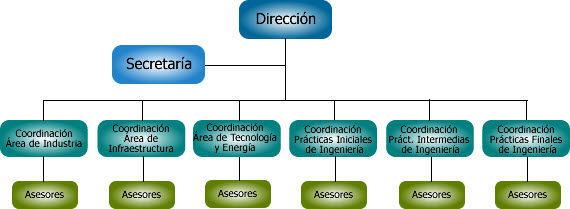
\includegraphics[width=1\linewidth]{images/201901-unidadeps-imagen01}
\figcaption{Organigrama Unidad de Prácticas de Ingeniería y EPS}

\end{minipage}

\end {flushleft}

\bigskip

\end {multicols}

\hypertarget{personal-administrativo-y-docente}{%
\section*{Personal Administrativo y Docente}\label{personal-administrativo-y-docente}}
\addcontentsline{toc}{section}{Personal Administrativo y Docente}

\begin{figure}[H]

{\centering 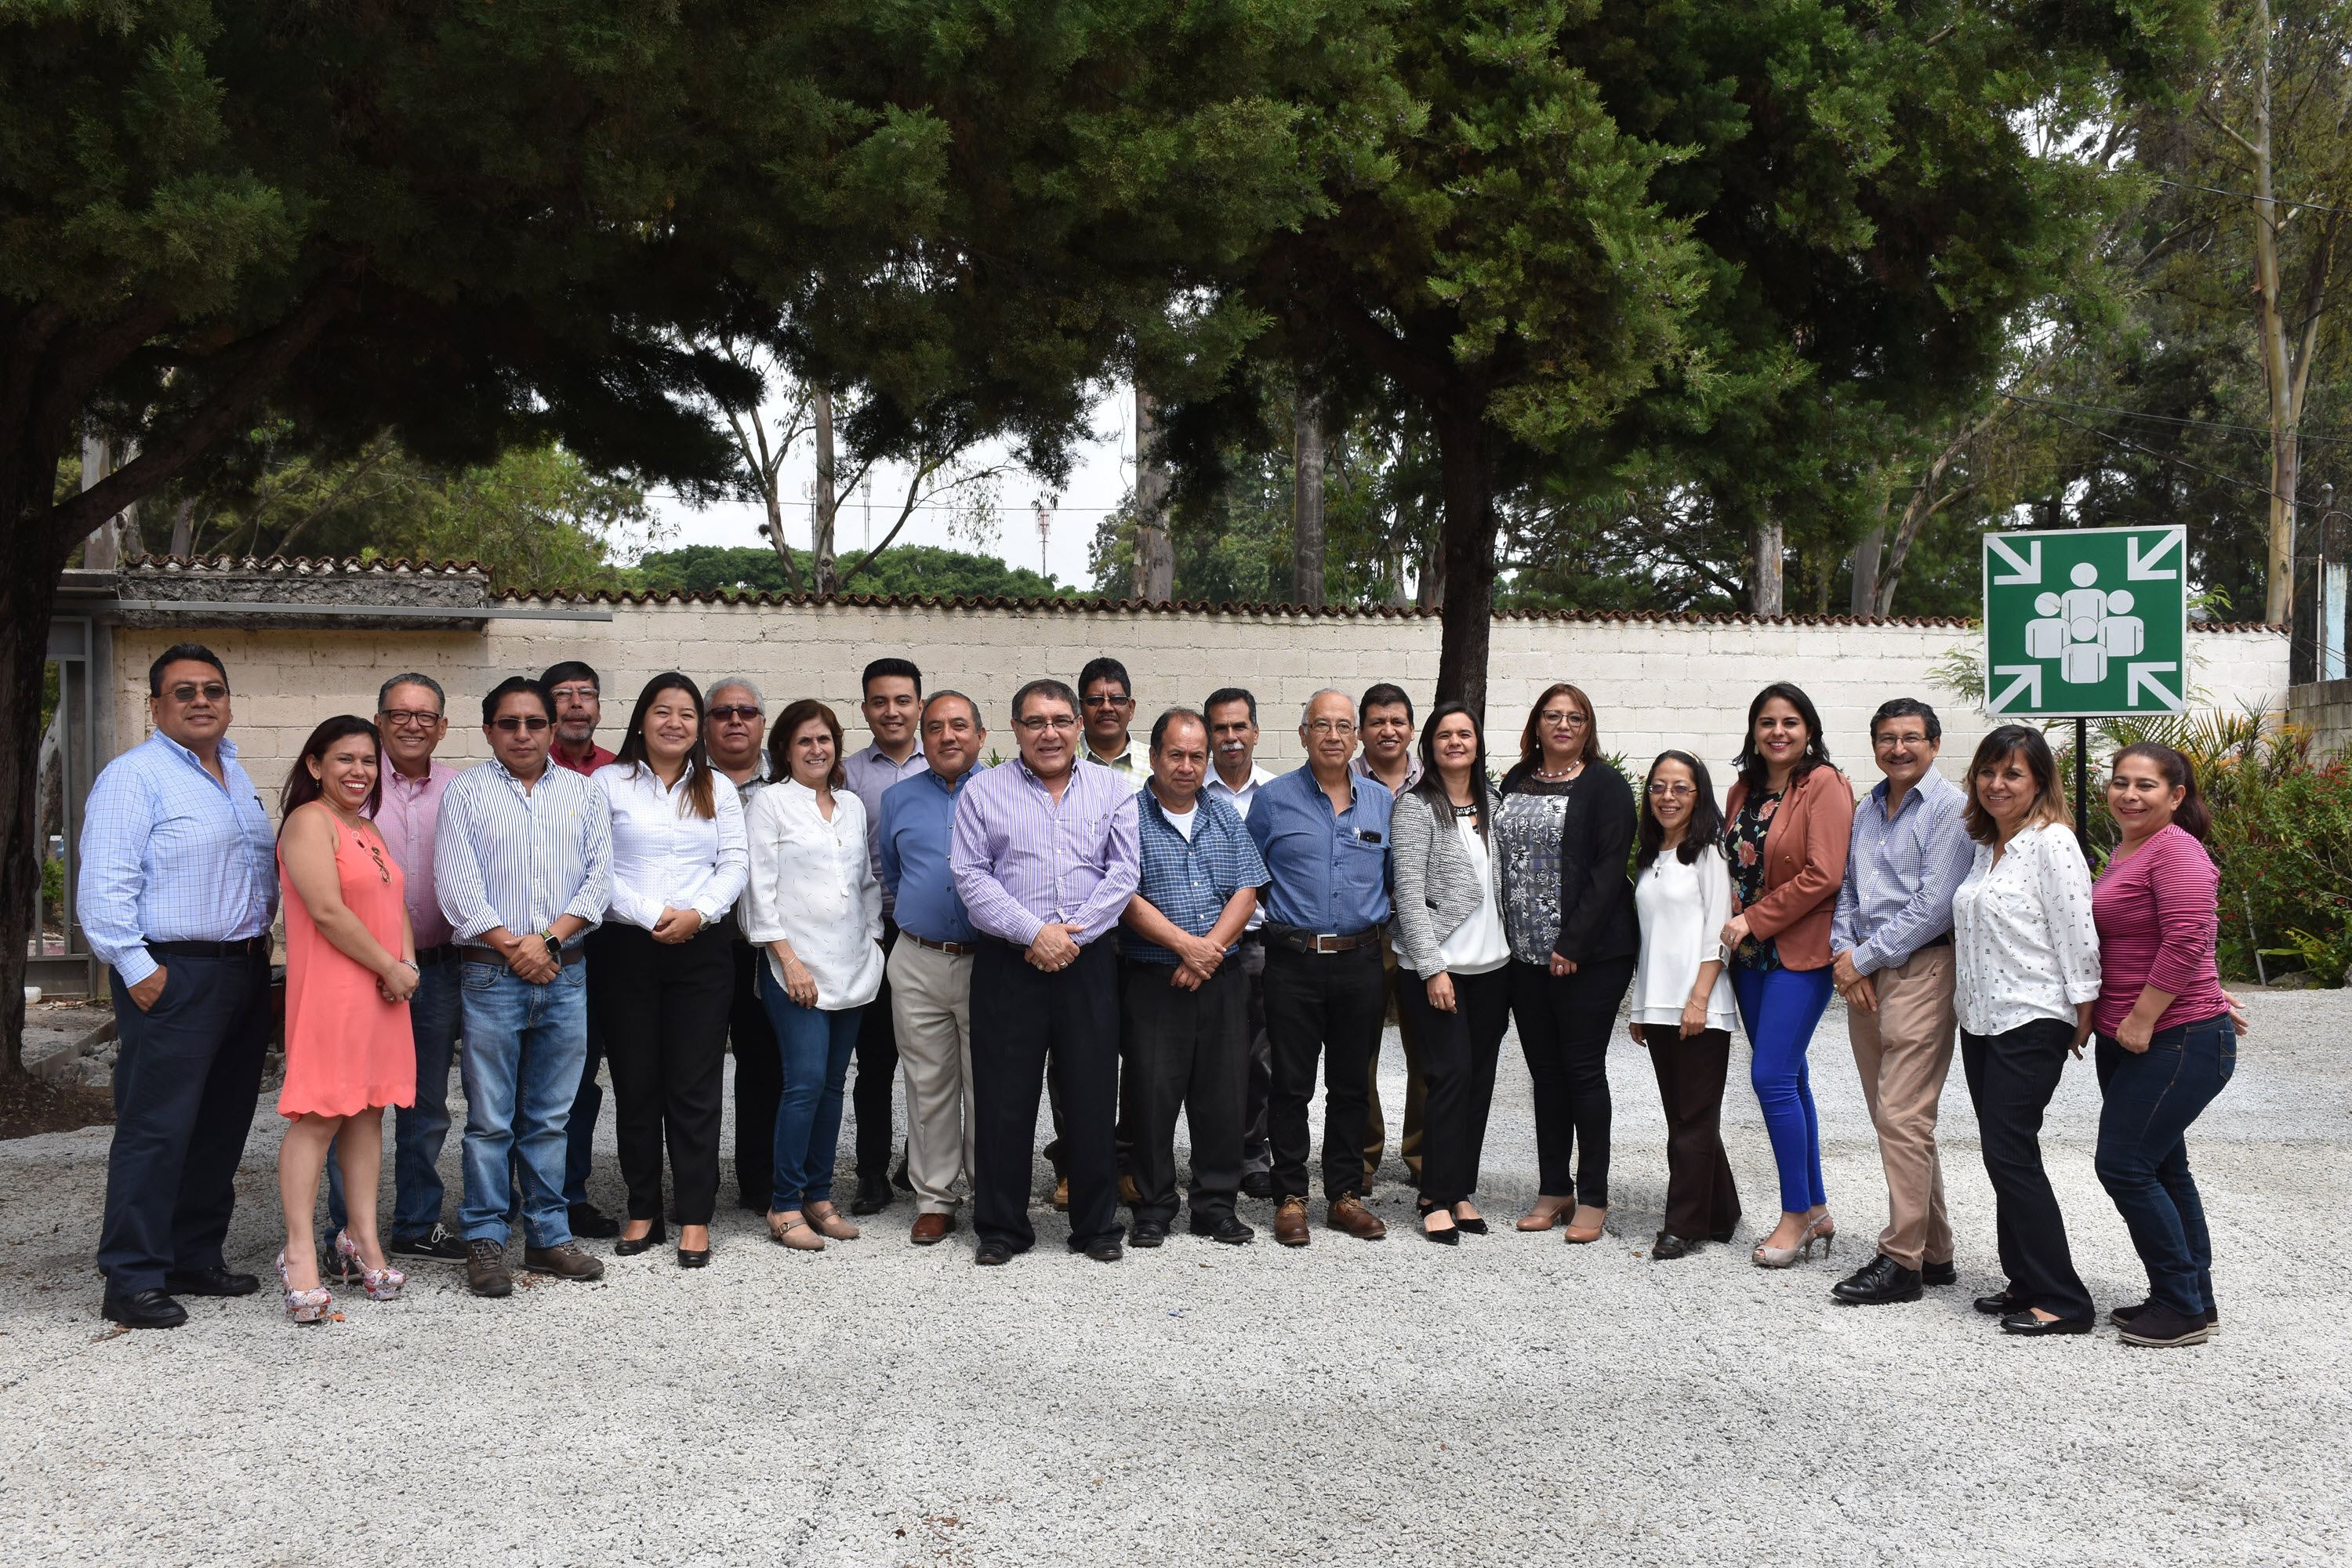
\includegraphics[width=0.78\linewidth]{images/201901-unidadeps-imagen02} 

}

\caption{Personal de Unidad de Prácticas de Ingeniería y Ejercicio Profesional Supervisado}\label{fig:unnamed-chunk-15}
\end{figure}

\hypertarget{descripciuxf3n-de-personal-administrativo-y-docente}{%
\section*{Descripción de Personal Administrativo y Docente}\label{descripciuxf3n-de-personal-administrativo-y-docente}}
\addcontentsline{toc}{section}{Descripción de Personal Administrativo y Docente}

\begin {multicols}{2}

A continuación nombres (izquierda a derecha):
\spacethreemilis

\begin{itemize}
\tightlist
\item
  Ingeniero Mecánico Emilio Vladimir Lux Monroy
  \spacetwomilis
\item
  Ingeniera Industrial Yocasta Ivanobla Ortíz del Cid
  \spacetwomilis
\item
  Ingeniero Civil Silvio José Rodríguez Serrano
  \spacetwomilis
\item
  Ingeniero Electricista Natanael Jonathan Requena Gómez
  \spacetwomilis
\item
  Ingeniero Mecánico Carlos Anibal Chicojay Coloma
  \spacetwomilis
\item
  Ingeniera Industrial Sindy Massiel Godinez Bautista
  \spacetwomilis
\item
  Ingeniero Civil Manuel Alfredo Arrivillaga Ochaeta
  \spacetwomilis
\item
  Ingeniera Civil Christa del Rosario Classon de Pinto
  \spacetwomilis
\item
  Ingeniero Mecánico Diego Israel Navarro Godinez
  \spacetwomilis
\item
  Ingeniero en Ciencias y Sistemas Sergio Leonel Gómez Bravo
  \spacetwomilis
\item
  Ingeniero Civil Oscar Argueta Hernández
  \spacetwomilis
\item
  Ingeniero Mecánico Edwin Estuardo Sarceño Zepeda
  \spacetwomilis
\item
  Ingeniero Civil Luis Gregorio Alfaro Véliz
  \spacetwomilis
\item
  Ingeniero Electricista Francisco Javier González López
  \spacetwomilis
\item
  Ingeniero Civil Juan Merck Cos
  \spacetwomilis
\item
  Ingeniero Químico Sergio Alejandro Recinos
  \spacetwomilis
\item
  Ingeniera Industrial Sigrid Alitza Calderón de León
  \spacetwomilis
\item
  Ingeniera Industrial Norma Ileana Sarmiento Zeceña de Serrano
  \spacetwomilis
\item
  Ingeniera Química Lorena Victoria Pineda Cabrera
  \spacetwomilis
\item
  Ingeniera Industrial Rocio Carolina Medina Galindo
  \spacetwomilis
\item
  Ingeniero Industrial Jaime Humberto Batten Esquivel
  \spacetwomilis
\item
  Ingeniera Civil Mayra Rebeca García Soria de Sierra
  \spacetwomilis
\item
  Licenciada en Administración de Empresas Maria Roxana Alvarado Monterroso
\end{itemize}

\end {multicols}

\medskip

\HRule

\medskip

\hypertarget{fgonzales}{%
\chapter{IEC 61850: Automatización de subestaciones eléctricas}\label{fgonzales}}

\begin{center}
\includegraphics[width=1\linewidth]{images/gonzalez} \end{center}

\begin {multicols}{2}

La importancia de la existencia de la Norma IEC 61850 radica en el impacto que tiene en la operación y control de subestaciones eléctricas, así como en la reducción de costos de instalación, operación y control.

Inicialmente destinada a subestaciones eléctricas, su aplicación se ha estado ampliando a Smart grid, autos eléctricos, sistemas Scada, sistemas de intercambio de información en tiempo real y energías renovables. O sea que su influencia es enorme y pronto será una herramienta de trabajo rutinaria e imprescindible en el sector eléctrico. Quienes se desempeñan en el área de potencia pronto serán invadidos por los nuevos conceptos que esta norma trae, siendo una oportunidad para integrar el trabajo en equipo de ingenieros electricistas e ingenieros electrónicos.

Especialistas en la norma consideran que quizá sea el proyecto más ambicioso en normalización realizado por la Comisión Electrotécnica Internacional IEC.

En una subestación tradicional la interoperabilidad entre dispositivos electrónicos inteligentes -IEDS- de diferentes marcas, así como el reemplazo de un dispositivo de determinada marca por otro de marca distinta requiere el cambio y adaptación de otros elementos, lo que presupone un gran esfuerzo de ingeniería y esquemas de trabajo complejos de integradores.

Otro tema importante en una subestación tradicional es el empleo de grandes cantidades de cableados de cobre para realizar señalización y control o intercambio de información entre los dispositivos inteligentes de la subestación; como consecuencia, por ejemplo, la subestación está limitada a esquemas de protección simples debido a la complejidad y costo del cableado. Al requerirse sistemas de protección más complejos, el cableado de cobre, que naturalmente se incrementa, implica mucho tiempo de ingeniería aplicada en el diseño y costos elevados de instalación y puesta en marcha. Además, la comunicación es limitada por los protocolos tradicionales y se incrementan los puntos de falla del sistema. Cuando el cobre se reemplaza por fibra óptica, es permitido por la IEC 61850 obtener una subestación eléctrica con sistemas más complejos, menos costosos, más veloces, y ocupando un espacio mínimo.

El objetivo principal de la norma IEC 61850 ha sido hallarle solución al problema de integración de los equipos electrónicos inteligentes de las subestaciones eléctricas pertenecientes a distintos fabricantes. Surge, entonces, por la necesidad de unificación de protocolos tanto estandarizados (IEC 60870-5-101, DNP3, MODBUS, entre otros) como propietarios, con el fin de obtener interoperabilidad entre los equipos de diferentes fabricantes y la facilidad y economía en su reemplazo. Es decir, que los grandes objetivos de la IEC 61850 son la interoperabilidad entre sí y la intercambiabiliad de equipos de distintos fabricantes, sin necesidad de cambiar otros elementos ni esfuerzos excesivos. Como objetivos secundarios, al utilizar fibra óptica, se logra una comunicación directa con los equipos primarios y una reducción sustancial del cableado tradicional sustituido por redes LAN.

Esta normativa parte de conceptos derivados de las nuevas técnicas de programación y telecomunicaciones, radicalmente diferentes a sus predecesoras y se estima tendrá una influencia en el sector eléctrico, mucho más allá de unos simples protocolos de comunicación, según los expertos.

\end {multicols}

\medskip

\HRule

\medskip

\hypertarget{article02}{%
\chapter{Áreas del pénsum de Ingeniería Industrial aplicadas en la práctica laboral}\label{article02}}

\begin{center}
\includegraphics[width=1\linewidth]{images/norma} \end{center}

\begin {multicols}{2}

\hypertarget{resumen}{%
\section{Resumen}\label{resumen}}

El pénsum de estudios de la carrera de ingeniería industrial de la Universidad de San Carlos de Guatemala (Usac) está integrado por tres áreas profesionales: Administración/Economía, Producción y Métodos Cuantitativos.

Los estudiantes de las diferentes carreras de la Facultad de Ingeniería al realizar las prácticas finales desarrollan proyectos relativos a los campos de aplicación de su especialidad. Durante el año 2020, en las prácticas finales de ingeniería industrial se asignaron 244 estudiantes, de los cuales 173 optaron a la modalidad de práctica laboral.

Con el fin de identificar las áreas del pénsum seleccionadas por los estudiantes de práctica laboral se analizó los proyectos realizados. El 29\% de los estudiantes elige proyectos del área Administración/ Economía, 56\% del área de Producción y 15\% del área de Métodos Cuantitativos.

\hypertarget{introducciuxf3n-1}{%
\section{Introducción}\label{introducciuxf3n-1}}

El programa de prácticas de ingeniería, de la Universidad de San Carlos de Guatemala (Usac) de acuerdo con el normativo vigente es: ``Una serie de actividades prácticas diseñadas en distintas modalidades, que forma parte del pénsum de estudios de la Facultad de Ingeniería de dicha casa de estudios, que tiene como misión formar estudiantes de Ingeniería con capacidad de aplicar los conocimientos, habilidades (destrezas) y criterios de su especialidad de acuerdo a su nivel académico, de tal forma que pueda confrontar los conocimientos teóricos con el mundo real y comprobar así su veracidad.''

Las prácticas finales forman parte del programa de
prácticas de ingeniería, son de carácter obligatorio
para todos los estudiantes de las diferentes
especialida-
des de la ingeniería que han aprobado
200 o más créditos académicos. Las tres opciones de
las prácticas finales de la Facultad de Ingeniería
son: Práctica Laboral, Docente y Empresarios
Juveniles.

El pénsum de la carrera de ingeniería industrial de la Facultad de Ingeniería de la Usac, está organizado por áreas: Administración/Economía, Producción y Métodos Cuantitativos. Los proyectos desarrollados por los estudiantes de prácticas finales en la modalidad laboral, corresponden a temas incluidos en las áreas del pénsum indicadas anteriormente.

\hypertarget{artuxedculo}{%
\section{Artículo}\label{artuxedculo}}

\hypertarget{materiales-y-muxe9todos}{%
\subsection{Materiales y métodos}\label{materiales-y-muxe9todos}}

Los objetivos del estudio son:

\begin{itemize}
\item
  Identificar las áreas del pénsum de ingeniería industrial consideradas en la práctica laboral.
\item
  Asociar los proyectos de práctica laboral con las áreas del pénsum de ingeniería industrial.
\end{itemize}

La fuente del estudio es documental y con alcance descriptivo. Se consultó la página web de la Facultad de Ingeniería y de la Escuela de Ingeniería Mecánica Industrial, para obtener el pénsum de estudios, analizar las áreas en que está dividido y los cursos que las integran. También se indagó en la plataforma virtual de la Unidad de Ejercicio Profesional Supervisado (EPS), para obtener el normativo de las prácticas de ingeniería. Además, se revisaron las bases de datos de las prácticas finales de los asesores docentes de la Unidad de EPS, del primer y segundo semestres del año 2020.

\begin {center}

\noindent\begin{minipage}[c]{\columnwidth}

\begin{center}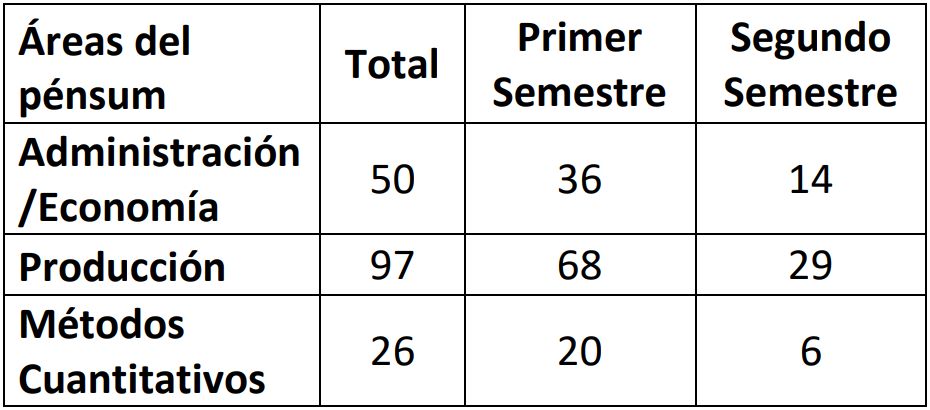
\includegraphics[width=1\linewidth]{images/02_03} \end{center}
\vspace{0.01cm}
\centering
\footnotesize

Tabla 3.1: Áreas del pénsum de ingeniería industrial aplicadas en las prácticas finales en el año 2020.

\end{minipage}

\end {center}

En la tabla 3.1 se puede observar que en el año 2020 se asignaron a la práctica laboral en el primer semestre 124 estudiantes y 49 en el segundo. De los proyectos realizados, 50 corresponden al área de Administración/Economía, 97 al área de Producción y 26 al área de Métodos Cuantitativos.

\begin {flushleft}
\noindent\begin{minipage}[c]{\columnwidth}

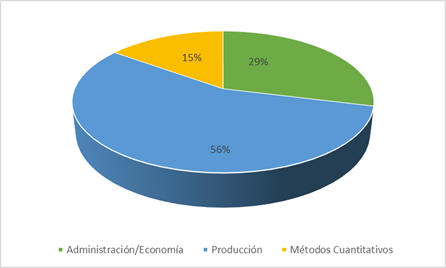
\includegraphics[width=1\linewidth]{images/02_02}
\figcaption{Áreas del pénsum de ingeniería industrial aplicadas en las prácticas finales en el año 2020.}

\end{minipage}

\end {flushleft}

En la figura 3.1 se observa que el 29\% de proyectos realizados son del área de Administración/Economía,
56\% del área de Producción y 15\% del área de Métodos Cuantitativos.

\hypertarget{conclusiones}{%
\section{Conclusiones}\label{conclusiones}}

Al analizar el pénsum de estudios de la carrera de ingeniería industrial se identificó que está
dividido en tres áreas: Administración/Economía, Producción y Métodos Cuantitativos. Las áreas
Administrativa/Economía y de Producción son las de mayor aplicación en los proyectos de
prácticas finales.

Al asociar los proyectos de prácticas finales con las áreas del pénsum de
ingeniería industrial se evidencia que el 29\% de los proyectos realizados por los estudiantes
corresponden al área Administración / Economía, 56\% al área de Producción y 15\% al área de Métodos
Cuantitativos.

\hypertarget{recomendaciones}{%
\section{Recomendaciones}\label{recomendaciones}}

Las autoridades de la Escuela de Ingeniería Mecánica Industrial y de la Unidad de EPS deben trabajar en conjunto para analizar las áreas del pénsum seleccionadas por los estudiantes de prácticas finales de ingeniería industrial y establecer estrategias para motivar el desarrollo de proyectos integrales.

\hypertarget{referencias}{%
\section{Referencias}\label{referencias}}

\begin{itemize}
\item
  {[}1{]} Unidad de Ejercicio Profesional Supervisado (EPS), \href{https://eps.ingenieria.usac.edu.gt/docs/Normativo_finales.pdf/}{\emph{Normativo del Programa de Prácticas de la Facultad de Ingeniería de la Universidad de San Carlos de Guatemala}}, 12 de abril de 2021. {[}En línea{]}. Disponible en: \url{https://bit.ly/3tA3UTC}. {[}Último acceso: 12 de abril de 2021{]}.
\item
  {[}2{]} Facultad de Ingeniería, USAC, {[}«Facultad de Ingeniería, USAC»{]}, \href{https://portal.ingenieria.usac.edu.gt/index.php/destacados-2/1294-redes-de-pensum/}{\emph{Facultad de Ingeniería, USAC.}}, 12 de abril de 2021. {[}En línea{]}. Disponible en: \url{https://bit.ly/394GSeh}. {[}Último acceso: 12 de abril de 2021{]}.
\item
  {[}3{]} EMI, {[}«EMI»{]}, \href{https://emi.ingenieria.usac.edu.gt/courses/area-administrativa/}{\emph{Cursos Área Administrativa.}}, 12 de abril de 2021. {[}En línea{]}. Disponible en: \url{https://bit.ly/2X9psKI}. {[}Último acceso: 12 de abril de 2021{]}.
\item
  {[}4{]} EMI, {[}«EMI»{]}, \href{https://eps.ingenieria.usac.edu.gt/docs/Normativo_finales.pdf/}{\emph{Cursos Área de Producción}}, 12 de abril de 2021. {[}En línea{]}. Disponible en: \url{https://bit.ly/3z54ry7}. {[}Último acceso: 12 de abril de 2021{]}.
\item
  {[}5{]} EMI, {[}«EMI»{]}, \href{https://emi.ingenieria.usac.edu.gt/courses/area-cuantitativa/}{\emph{Cursos Área Cuantitativa}}, 12 de abril de 2021. {[}En línea{]}. Disponible en: \url{https://bit.ly/3hosFx6}. {[}Último acceso: 12 de abril de 2021{]}.
\end{itemize}

\end {multicols}

\medskip

\HRule

\medskip

\hypertarget{article03}{%
\chapter{EPS, una experiencia diferente}\label{article03}}

\begin{center}
\includegraphics[width=1\linewidth]{images/glenda} \end{center}

\begin {multicols}{2}

\hypertarget{resumen-1}{%
\section{Resumen}\label{resumen-1}}

El EPS es una modalidad de graduación por la que muchos estudiantes optan, ya que la misma significa experiencia y compromiso; para muchos es un comienzo o una nueva etapa y al ser desconocida nos hacemos diferentes interrogantes sobre en qué consiste el EPS y por qué optar por esta modalidad. Pues bien, en el presente artículo se redacta la experiencia de una estudiante de EPS y los proyectos que se desarrollaron: dos sistemas de drenaje y a su vez una serie de recomendaciones para futuros epesistas.

\hypertarget{introducciuxf3n-2}{%
\section{Introducción}\label{introducciuxf3n-2}}

La Facultad de Ingeniería permite optar por diferentes modalidades para llegar a la tan anhelada graduación, pero\ldots{} ¿Por qué optar por el ejercicio profesional supervisado (EPS)? Pues bien, el deseo de aprender desde la práctica, experiencia, hacer algo por la comunidad fue lo que me llevó a elegir esta metodología. Sin embargo, el camino no fue fácil: el inicio de una pandemia, un cambio en la modalidad, terrenos no explorados, por decirlo más coloquialmente, y terminar dos proyectos sin el apoyo directo de la municipalidad como se tenía previsto debido al distanciamiento social, sin duda dificultó todo.

Es importante resaltar que cuando te dispones a realizar el diseño de los proyectos lo que ves en los cursos es solo una cuarta parte de la información que se requiere. A un inicio me invadió la incertidumbre de cómo comenzar, y conforme iba avanzando surgían más vacíos que anteriormente no sabía que existen; pero eso es lo interesante del EPS, que al final llenas todas esas lagunas y cualquiera que sea el tema que se elija, sin duda se aprende a manejarlo a la perfección. Y si te preguntas cómo lo logré, a continuación, te expondré los proyectos que tuve asignados y además te contaré los obstáculos, dificultades que pasé, así como consejos y soluciones que espero te sirvan.

\hypertarget{artuxedculo-1}{%
\section{Artículo}\label{artuxedculo-1}}

\hypertarget{el-problema}{%
\subsection{El problema}\label{el-problema}}

En la modalidad de EPS se establece un período de tiempo para realizar un diagnóstico de las necesidades de la población; la municipalidad brinda la información necesaria y con ella se realiza un listado de prioridades; se selecciona la más urgente y que su solución signifique un aporte apremiante hacia la comunidad. En mi situación, opté por el diseño de un drenaje sanitario y un drenaje pluvial, ya que los actuales se encontraban obsoletos; además, una falla que atraviesa el lugar ocasionó que los pozos y tuberías se desplomaran; adicionalmente, las aguas sanitarias no estaban siendo tratadas, lo que causaba gran contaminación en el área.

\hypertarget{diseuxf1o-de-los-proyectos}{%
\subsection{Diseño de los proyectos}\label{diseuxf1o-de-los-proyectos}}

El inicio del proyecto consiste en buscar qué se necesita y cómo se va a desarrollar. Los factores importantes para el diseño de drenajes son: topografía, población, características climatológicas, entre otras. Una vez obtenida esa información se puede comenzar con el desarrollo; para esto se busca apoyo en libros, cuadernos de los cursos que aplicaban al proyecto, tesis y lo más importante, las NORMAS, ya que se sabe que en la ingeniería civil constituyen el fundamento para el diseño de cualquier proyecto.

Seguido de eso se procede a la realización del proyecto; en el caso de drenajes una hoja en Excel facilita todo el cálculo. Se deben considerar las normas y fórmulas, y establecer un orden para el ingreso de datos; los cálculos se realizan automáticamente. Otro programa que será de mucha utilidad es Civil 3D, aquí sí importa la topografía, se trazan calles, viviendas y el sistema de drenaje como tal. Si no se sabe cómo utilizar el programa para crear la plantilla de drenaje, en YouTube hay un video completo con la información para crear la plantilla, el trazo de la línea y perfiles.

Ahora bien, la parte difícil cuando se desconoce del tema y que en lo personal me creó dificultad es cómo utilizar los datos que me da Civil 3D e introducirlos a Excel y viceversa. Una vez que la línea de drenaje está trazada, se tienen las cotas de terreno que se muestran por defecto y se debe trazar una cota para medir la distancia; con ello se obtienen pendientes. Posteriormente se cuentan las viviendas por tramo, se introducen los datos al Excel junto con la información adicional que puede darte la municipalidad y ya se tiene el cálculo del cual se obtienen las cotas invert, y en ``propiedades'' se sustituye la información; estos en el caso de un drenaje sanitario. Para el drenaje pluvial se trabaja de la misma manera, con la diferencia de que, en vez de contar viviendas, se deben trazar trapecios y con el comando área medirlo e introducir los datos al Excel.

\hypertarget{soluciones}{%
\subsection{Soluciones}\label{soluciones}}

\begin{itemize}
\tightlist
\item
  Desarrollar el diseño de un sistema de drenaje que se conecte a una planta de tratamiento y evitar contaminación en el área.
\item
  Desarrollar el diseño de un sistema de drenaje pluvial que desfogue al río más cercano y con ello evitar daños a viviendas, carreteras, entre otros.
\end{itemize}

Pues bien, una vez que expuse en qué consiste el diseño de los proyectos, a continuación, desarrollaré una serie de recomendaciones con base en la experiencia que obtuve en el EPS.

\hypertarget{recomendariones}{%
\section{Recomendariones}\label{recomendariones}}

\begin{itemize}
\item
  Si se realiza el proyecto desde casa, lo primero que se aconseja es no entrar en pánico y no dejar que gane el estrés. Debe pedirse ayuda a cualquier amigo que vaya más adelantado o que conozca más del tema y si no hay alguien que pueda apoyar de las personas más cercanas, está el asesor de tesis, que seguro sabrá cómo dar una solución.
\item
  Revisar constantemente cada cosa que se realice; el proyecto es una cadena y si se comete error en un dato, lo demás que se realice estará malo. OJO, con esto no me refiero a que dudes de lo que estás haciendo, sino que le prestes atención y el tiempo que requiera.
\item
  El proceso puede ser largo y generar incertidum-
  bre, más cuando por la pandemia se trata de una nueva experiencia en EPS, pero al final todo tiene una salida y tarde o temprano si el estudiante se lo propone, terminará todo el proceso satisfactoriamente.
\end{itemize}

\hypertarget{referencias-1}{%
\section{Referencias}\label{referencias-1}}

\begin{itemize}
\tightlist
\item
  {[}1{]} Instituto de Fomento Municipal, \href{https://bit.ly/39x9Bc5}{\emph{Normas generales para el diseño de alcantarillados. Guatemala: INFOM. 76 p}}.
\end{itemize}

\end {multicols}

\medskip

\HRule

\medskip

\hypertarget{article08}{%
\chapter{Accesibilidad en uso de plataforma virtual en la Escuela de Postgrado, FAHUSAC}\label{article08}}

\begin{center}
\includegraphics[width=1\linewidth]{images/claudia} \end{center}

\begin {multicols}{2}

\hypertarget{resumen-2}{%
\section{Resumen}\label{resumen-2}}

En esta época en que debido a la crisis sanitaria se deben superar todos los obstáculos para consolidar la educación superior, surge la interrogante: ¿cuáles son las condiciones y facilidades de acceso a la plataforma virtual que han tenido los estudiantes de las diferentes maestrías de la Escuela de Estudios de Posgrado de la Facultad de Humanidades en el primer semestre del año 2020? Con base en esa inquietud se realizó una investigación no experimental, transeccional, relacionada con el área tecnológica, que permitió recabar datos de índole personal, social, económica, laboral y cultural, respecto de las condiciones de accesibilidad y uso de la plataforma virtual a la cual pueden ingresar los estudiantes. La técnica utilizada para la recolección de la información fue la encuesta; esta fue compartida a través de formulario de Google, con una muestra 112 estudiantes del primer ciclo de las diferentes carreras de maestrías que ofrece la Escuela de Estudios de Postgrado, la cual fue seleccionada para el estudio en mención.

Los resultados indicaron que un 40 \% de estudiantes no recibe suficiente información sobre la utilización de las herramientas disponibles en la plataforma virtual de la Escuela de Estudios de Postgrado, y un 49 \% que no reciben información de la interfaz de la plataforma virtual de la misma Escuela.

Se elaboró una guía sobre la utilización de la plataforma virtual de la Escuela de Postgrado, considerando el contexto de la escuela y la plataforma institucional para lograr su pertinencia con el uso de las herramientas de las que pueden disponer los estudiantes de los diferentes programas de maestrías que ofrece la Escuela de Estudios de Postgrado.

\hypertarget{introducciuxf3n-3}{%
\section{Introducción}\label{introducciuxf3n-3}}

El uso de las nuevas tecnologías informáticas de comunicación -TIC-, permite acortar distancias,
y atender de diferentes modalidades a los sujetos; en el ámbito educativo, en las plataformas
virtuales, se dispone de una serie de recursos y actividades que permiten desarrollar el proceso
de enseñanza aprendizaje. Al revisar teoría relacionada con la educación virtual, pudo apreciarse
la incidencia en definirla como una estrategia educativa que facilita el manejo de la información
y permite la aplicación de nuevos métodos pedagógicos enfocados al desarrollo de aprendizajes
significativos, los cuales están centrados en el estudiante y en su participación dinámica
(Enciclopedia Cubana en la Red {[}EcuRed{]}, 2019).

\hypertarget{artuxedculo-2}{%
\section{Artículo}\label{artuxedculo-2}}

Los programas de Maestría son impartidos en las modalidades e-learning y b-learning a través
de plataforma Moodle. Actualmente hay bastantes ventajas con el uso de herramientas digitales
para acortar distancias de comunicación que favorezcan el desarrollo personal y profesional. En
el contexto de la Escuela de Postgrado de la Facultad de Humanidades, con estas herramientas
se privilegia la atención en docencia en modalidad virtual utilizando diferentes dispositivos,
acceso a la información en tiempo y forma, y facilidad de ingreso en cualquier lugar y espacio.
Sin embargo, se ha observado que los estudiantes presentan una serie de dificultades de
accesibilidad a la plataforma, así como, en la utilización de los recursos y actividades disponibles
en la misma; situación que repercute negativamente en su proceso de aprendizaje. Asimismo,
las Tecnologías de la Información y Comunicación -TIC-, son tecnolo-
gias que han beneficiado a
los estudiantes y docentes porque acortan distancias y tiempo, obteniendo como resultado el
acceso de la información para realizar las actividades de forma virtual a través de la plataforma
de la Escuela de Postgrado. Por lo antes, expuesto surgió la interrogante ¿Cuáles son las condiciones
y facilidades de acceso a la plataforma virtual, que tienen los estudiantes de Maestría
en Currículum, Maestría en Docencia Universitaria, Maestría en Docencia Universitaria con
Énfasis en Tecnologías y Maestría en Investigación, en el plan de los días sábado y domingo y
en modalidad virtual, en la accesibilidad, utilización de los recursos y actividades de la plataforma
Moodle de la Escuela de Estudios de Postgrado de la Facultad de Humanidades, en el primer
semestre del 2020.

Los programas de aprendizaje llevados en modalidad virtual se utilizan en todos los niveles
educativos y especialmente en la educación superior. La Escuela de Estudios de Postgrado de
la Facultad de Humanidades sirve programas de maestría y doctorado en modalidad
semipresencial, es decir b-learning. De acuerdo con Ruiz (2011), la definición de las variantes de
modalidad virtual se resume en:

El blended learning (b-Learning) sigue avanzando en el contexto internacional como una
alternativa frente a la modalidad de la educación completamente virtual (e-Learning) como una
opción de mejoramiento de la calidad de la instrucción respecto de la modalidad de educación
tradicional, tanto presencial como a distancia y la formación laboral corporativa. (p.~11)

La importancia del presente estudio radica en los datos que se obtuvieron en las áreas de índole
personal, social, económico, laboral y cultural, relacionados con el área tecnológica, sobre las
condiciones de accesibilidad y uso de la plataforma virtual que presentan los estudiantes.
El objetivo general de la investigación se centró en identificar las condiciones y accesibilidad a la
plataforma virtual, que tienen los estudiantes de Maestría en Currículum, Maestría en Docencia
Universitaria, Maestría en Docencia Universitaria con Énfasis en Tecnologías y Maestría en
Investigación, en el plan de estudio de los días sábado y domingo, y en modalidad virtual de la
Escuela de Estudios de Postgrado, Facultad de Humanidades, en el primer semestre del 2020.

Los objetivos específicos se enfocaron en:

\begin{itemize}
\item
  Establecer los requisitos básicos de conectividad a la plataforma virtual que tienen los
  estudiantes de los programas de objeto de estudio de la Escuela de Estudios de Postgrado,
  planes de los días sábado y domingo y en modalidad virtual.
\item
  Enumerar los recursos de la plataforma virtual más utilizados por los estudiantes en su
  proceso de aprendizaje-enseñanza.
\item
  Describir las actividades de la plataforma que utilizan los estudiantes de los diferentes
  programas de maestrías en su proceso de aprendizaje.
\item
  Elaborar una guía para el uso de la plataforma virtual dirigida a los estudiantes de los
  programas de Maestría de la Escuela de Estudios de Postgrado, Facultad de Humanidades
  de la Universidad de San Carlos de Guatemala.
\end{itemize}

El estudio fue realizado con la finalidad de explorar las condiciones y facilidades de acceso a la
plataforma virtual, cuyos resultados sirvieron para conocer mejor el fenómeno de investigación.
Con base en los objetivos planteados se trabajó con un diseño transeccional o transversal que
recolectó datos en un solo momento, sin manipular las variables, con estudiantes inscritos en el
año 2020 en el primer ciclo, en los diferentes programas de maestría

Resultados de la encuesta aplicada:

\begin{center}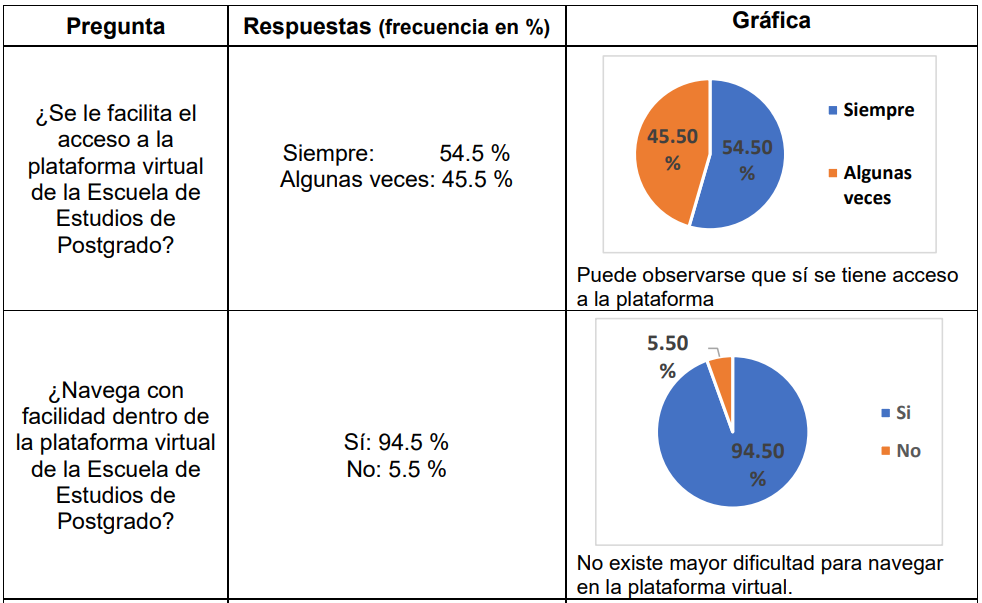
\includegraphics[width=1\linewidth]{images/09_03} \end{center}

\begin{center}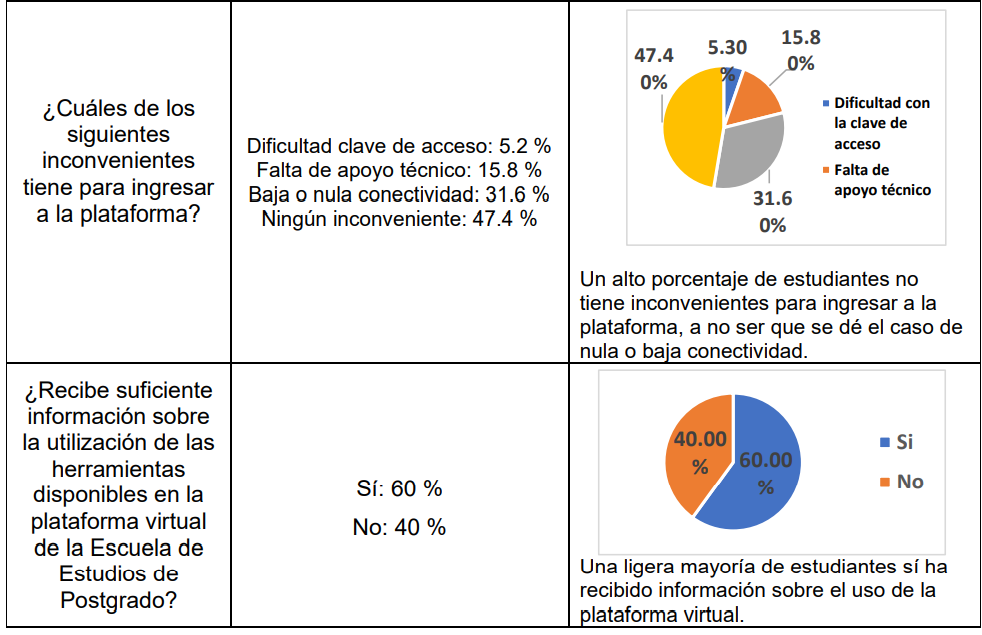
\includegraphics[width=1\linewidth]{images/09_02} \end{center}

\begin{center}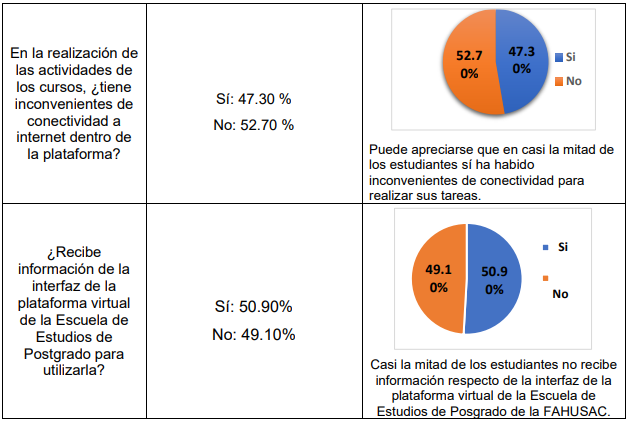
\includegraphics[width=1\linewidth]{images/09_04} \end{center}

\hypertarget{conclusiones-1}{%
\section{Conclusiones}\label{conclusiones-1}}

\begin{itemize}
\item
  Es aceptable la accesibilidad para el ingreso a la plataforma virtual por parte de los
  estudiantes, ya que tienen la opción de hacerlo en diferentes horarios. De manera general,
  sí se les facilita el acceso a los contenidos de los cursos.
\item
  Los estudiantes de primer ciclo de los diferentes programas de maestría sí tienen facilidad
  para navegar dentro de la plataforma de la Escuela de Estudios de Posgrado de la Facultad
  de Humanidades; solo el 5.5 \% respondió lo contrario.
\item
  Es importante que dentro de las plataformas virtuales haya conectividad estable para que
  los estudiantes no tengan inconvenientes; un 47.3 \% reportó que sí tuvieron dificultades al
  realizar las actividades asignadas por los docentes.
\item
  Como resultado del trabajo de investigación se encontró la necesidad de elaborar una guía
  para el uso de la plataforma virtual dirigida a los estudiantes de la Escuela de Postgrado de
  la Facultad de Humanidades de la Universidad de San Carlos de Guatemala; para ello se
  consideró el contexto de la Escuela y la plataforma institucional; de esa manera se espera
  lograr su pertinencia respecto de la disposición y uso de las herramientas apropiadas.
\end{itemize}

\hypertarget{recomendaciones-1}{%
\section{Recomendaciones}\label{recomendaciones-1}}

A las autoridades de la Escuela de Estudios de Postgrado:

\begin{itemize}
\item
  Promover capacitaciones sobre el uso de la plataforma virtual, acceso y optimización, tanto
  para estudiantes de primer ingreso como para docentes de la Escuela de Estudios de
  Postgrado de la Facultad de Humanidades de la Universidad de San Carlos de Guatemala.
\item
  Gestionar una mejor conectividad en la plataforma virtual para evitar los inconvenientes que
  puedan darse cuando los estudiantes realicen sus actividades.
\item
  Implementar el uso de la Guía para utilizar la plataforma virtual de la Escuela de Estudios
  de Postgrado de la Facultad de Humanidades-USAC.
\end{itemize}

A los docentes de la Escuela de Estudios de Postgrado:

\begin{itemize}
\tightlist
\item
  Promover el trabajo colaborativo entre los estudiantes a través de las actividades
  planificadas en los diferentes cursos de la Escuela de Estudios de Postgrado, para
  socializar y fortalecer el aprendizaje.
\end{itemize}

\hypertarget{referencias-2}{%
\section{Referencias}\label{referencias-2}}

\begin{itemize}
\item
  {[}1{]} {[}«Acuña, M. »{]}, \href{http://elearningmasters.galileo.edu/2017/10/17/tecnicas-y-estrategias-de-ensenanza-virtual/}{\emph{ATécnicas y estrategias de enseñanza virtual e-Learning Másteres }}, 2017. {[}En línea{]}. Disponible en: \url{https://bit.ly/3AaXf48} .
\item
  {[}2{]} {[}«Departamento de Educación Virtual FAHUSAC.»{]}, \href{https://www.youtube.com/watch?v=vh2v8cn8920}{\emph{Video tutorial de 3 estudiantes. Entrega de tarea, Facultad de Humanidades, USAC. Guatemala. Videos tutoriales para uso de campus virtual FAHUSAC}}, 26 de marzo de 2020. {[}En línea{]}. Disponible en: \url{https://bit.ly/3mpjhey}.
\item
  {[}3{]} {[}«Díaz, D.»{]}, {[}\emph{Tic en educación superior: ventajas y desventajas. Revista Educación y Tecnología. Número 4, pp.~44-50.}{]} (2013).
\item
  {[}4{]} {[}«EcuRed Contributors»{]}, \href{https://www.ecured.cu/index.php?\%20title=Investigaci\%C3\%B3n_no_experimental\&oldid=1451545.}{\emph{Investigación no experimental. Enciclopedia Cubana en la Red}}, 2012. {[}En línea{]}. Disponible en: \url{https://bit.ly/3Adw4Wb}.
\item
  {[}5{]} {[}«EcuRed Contributors»{]}, \href{https://www.ecured.cu/index.php?title=\%20Educaci\%C3\%B3n_Virtual\&oldid=3417611}{\emph{Educación Virtual. Enciclopedia Cubana en la Red.}}, 2019. {[}En línea{]}. Disponible en: \url{https://bit.ly/3iBmJ4J}.
\item
  {[}6{]} {[}«Ruiz C.»{]}, {[}\emph{Tendencias actuales en el uso del B-Learning: un análisis en el contexto del Tercer Congreso Virtual Iberoamericano sobre la Calidad en Educación a Distancia (\href{mailto:EduQ@2010}{\nolinkurl{EduQ@2010}}) Investigación y Postgrado, vol.~26, núm. 1, enero-abril. pp.~9-30 Venezuela: Universidad Pedagógica Experimental Libertador.}{]}.
\item
  {[}7{]} {[}«Facultad de Humanidades»{]}, \href{http://www.humanidades.usac.\%20edu.gt/usac/postgrado/}{\emph{Educación Virtual. Enciclopedia Cubana en la Red.}}( Escuela de Estudios de Postgrado, Universidad de San Carlos de Guatemala), 2014. {[}En línea{]}. Disponible en: \url{https://bit.ly/3Fjikx6}.
\end{itemize}

\end {multicols}

\medskip

\HRule

\medskip

\hypertarget{article04}{%
\chapter{Transformación digital}\label{article04}}

\begin{center}
\includegraphics[width=1\linewidth]{images/rainman} \end{center}

\begin {multicols}{2}

\hypertarget{introducciuxf3n-4}{%
\section{Introducción}\label{introducciuxf3n-4}}

En la Facultad de Arquitectura de la Universidad de San Carlos, como en la mayoría de las demás Facultades, existen procesos para la realización de solicitudes a sus correspondientes Juntas Directivas. En la mayoría de estas, el proceso en mención es todavía manual, a través del cual el interesado debe presentarse en las oficinas a llenar un formulario para la solicitud, y luego consultar su estado o avance periódicamente.

Este proceso requiere una gran inversión de recursos por parte del personal administrativo para recibir, planificar y darle resolución a las solicitudes. Es aquí donde nace la nacesidad de realizar una transformación digital para optimizar el uso de recursos, y facilitar la experieancia a los solicitantes (usuarios) durante este proceso.

\hypertarget{artuxedculo-3}{%
\section{Artículo}\label{artuxedculo-3}}

De acuerdo con Salesforce (2005), la transformación digital es el proceso de usar tecnología digital para crear (o modificar uno existente) cualquier proceso de negocio, cultura y experiencias de usuario para alcanzar los requerimientos de un mercado cambiante.

La palabra mercado en la definición anterior no hace referencia únicamente a las instituciones que se dedican a vender un producto a servicio, realmente aplica para cualquier institución en general. Instituciones con las distintas Facultades dentro de nuestra universidad también están compuestas por procesos, muchos de estos definidos desde hace mucho tiempo atrás, y que persisten hasta la fecha. Se ha llegado a los días donde surge la necesidad de dar el paso hacia la transformación digital, y adaptarse a una nueva cultura para mejorar la experiencia de usuarios, lo cual abarca a toda una comunidad estudiantil.

Como parte del Ejercicio Profesional Supervisado, se tuvo la oportunidad de colaborar con la transforma-
ción que la Facultad de Arquitectura decidió dar en su proceso de recepción, planifiación y resolución de solicitudes a Junta Directiva.

Para esto, el primer paso consistió en entender el proceso actual, el cual consistía en que el solicitante se presenta a la recepción de la Facultad, llena el formulario y adjunta los documentos correspondientes; la secretaria recibe y categoriza las solicitudes y las ordena por prioridad. Luego de unos días de haber recibido solicitudes, se hace la planificación de la agenda, la cual contiene el listado de solicitudes que serán revisadas por los miembros de Junta Directiva en su próxima sesión. La agenda es notificada a todos los miembros y cuando la fecha de celebración de Junta Directiva se da, la sesión es efectuada y se da resolución a todas las solicitudes presentadas en la agenda.

Para esto las secretarias se apoyan de plantillas en Google Docs elaboradas por ellas, y toda la información es almacenada en documentos de Google Drive. Son las secretarias quienes se encargan de transcribir documentos, redactar las actas con las resoluciones y enviar las notificaciones. Esto es un proceso manual que requiere de mucho tiempo para ser realizado.

En este proceso se pudo observar el mal uso de recursos, la existencia de muchas tareas repetitivas y una desorganización total en almacenamiento y manejo de la información. Con base en lo anterior, se desarrolló una propuesta, en la cual se resaltan las siguientes características:

\begin{enumerate}
\def\labelenumi{\alph{enumi}.}
\item
  Disponibilidad: la información debe estar disponible todo el tiempo, es decir, se deben realizar solicitudes desde cualqier lugar
  y cualquier hora.
\item
  Estandarización: los procesos deben estar definidos y estandarizados; se deben realizar de la misma forma; esto lleva a la creación
  de un sistema donde las secretarias puedan realizar todas las tareas requeridas.
\end{enumerate}

Una vez indentificados los procesos, su necesidad de organización y estandarización, más la necesidad de la disponibilidad, fue fácil concluir que se estaba ante un caso de Transformación Digital.

La fase anterior consistió en un conjunto de reuniones, intercambio de correos y observación de los procesos; se trató de una fase de análisis como todo problema de ingeniería; esta siempre es la parte más importante, pues con base en ella puede plantearse una solución correcta que cumpla con las expectativas requeridas.

Pues bien, la solución propuesta fue un sistema orientado a servicios, los cuales se encargarían de realizar todas las tareas relacionadas con la recepción, planificaicón y resolución de solicitudes. Los servicios permiten ser consumidos por cualquier aplicación, esto permitiría integrar el sistema con plataformas existentes como el portal de catedráticos, estudiantes, entre otros, así como las plataformas futuras; con esto se cubrió la disponibilidad.

También se desarollaría una aplicación web que consumiría los servicios y sería la única herramienta por utilizar para la planificación y resolución de las solicitudes; con esto se atendió la estandarización.

El sistema permitiría tener toda la información centralizada, a partir de la cual se podrían automatizar tareas, tales como la generación de transcripciones y actas. Serviría de soporte para la planificaicón de la agenda, el envío de convocatorias, entre otras.
El sistema hace uso también de los servicios de Google para el manejo de archivos adjuntos, generación de documentos de actas, transcripciones y envíos de correo.

Entre las ventajas del sistema se encuentran: estructura de la información, la información ahora se encuentra centrazlizada, es integra y cuenta con alta disponibilidad; automatización, muchas de las tareas antes realizadas manualmente, son ahora realizadas automáticamente, reduciento el tiempo que se invertía en estos procesos; seguridad, ahora se tiene registro del acceso a la información, se cuenta con permisos que garantizan que solo las personas adecuadas pueden realizar las modificaciones permiti-
das; así también se han auditado las actividades involucradas en los procesos; por último, la reutiliza-
ción, el sistema es configurable y parametrizable, para que pueda ser utilizado por otras unidades académicas que también quieran dar el paso a la transformación digital.

\begin {flushleft}
\noindent\begin{minipage}[c]{\columnwidth}

\centering

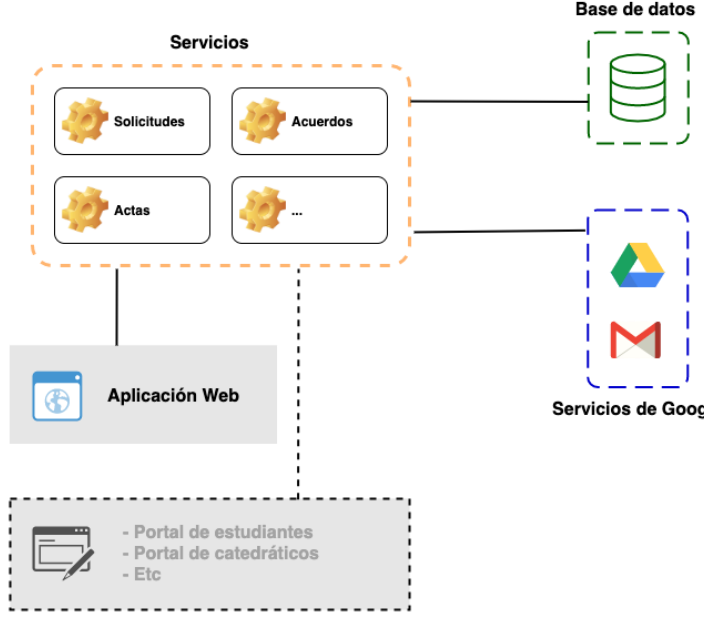
\includegraphics[width=0.75\linewidth]{images/04_02}
\figcaption{Diagrama de Arquitectura. Fuente: elaboración propia}

\end{minipage}

\end {flushleft}

\hypertarget{conclusiones-2}{%
\section{Conclusiones}\label{conclusiones-2}}

\begin{itemize}
\item
  La transformación digital ofrece a las instituciones optimizar sus recursos, así como mejorar la experiencia de sus usuarios.
\item
  La transformación digital es una necesidad para satisfacer las demandas actuales.
\item
  Es importante realizar un buen análisis antes de proceder a la resolución de un problema de ingeniería de Software.
\end{itemize}

\hypertarget{referencias-3}{%
\section{Referencias}\label{referencias-3}}

\begin{itemize}
\tightlist
\item
  {[}1{]} Salesforce, \href{https://www.wiley.com/en-us}{«Salesforce»}, \href{https://www.ugr.es/~filosofia/recursos/\%20innovacion/convo-2005/trabajo-escrito/como-elaborar-un-articulcientifico.html}{\emph{What is Digital Transformation}}, 2005. {[}En línea{]}. Disponible en: \url{https://bit.ly/3EaYjbu}. {[}Último acceso: 30 de abril de 2021{]}.
\end{itemize}

\end {multicols}

\medskip

\HRule

\medskip

\hypertarget{article05}{%
\chapter{Instalación y configuración del sistema Koha para la Facultad de Medicina Veterinaria y Zootecnia}\label{article05}}

\begin{center}
\includegraphics[width=1\linewidth]{images/edson} \end{center}

\begin {multicols}{2}

\hypertarget{resumen-3}{%
\section{Resumen}\label{resumen-3}}

El proyecto realizado en la Facultad de Veterinaria se basó en la instalación y configuración del sistema administrativo de bibliotecas KOHA, el cual ofrece una plataforma para la administración de la biblioteca, destinada para los empleados de la biblioteca, así como un sitio para los usuarios públicos como estudiantes y público en general.

La biblioteca de veterinaria ya contaba con una instancia de Koha, pero a lo largo del tiempo y la no correcta configuración del sistema provoco que el sistema se volviera lento e inestable, dando una experiencia no satisfactoria al usuario, por lo que a la nueva instancia se migro toda la información tanto de los elementos bibliográficos como de los usuarios.

Un punto para mencionar es la personalización del sitio público con la imagen institucional el cual involucro modificación de plantillas, hojas de estilo y código de JavaScript, además de entregar documentación sobre el uso de los módulos del sistema.

\hypertarget{introducciuxf3n-5}{%
\section{Introducción}\label{introducciuxf3n-5}}

La biblioteca de la Facultad de Medicina Veterinaria y Zootecnia de la Universidad de San Carlos de Guatemala contaba con una instancia del sistema administrativo KOHA la cual ayuda a la gestión y control de procesos y recursos pertenecientes a dicha institución.

Los objetivos del proyecto fueron: migrar la instancia anterior de KOHA a una versión reciente, por lo cual se necesitaba instalar y trasladar información del sistema anterior a una nueva versión, personaliza-
ción de las páginas a la imagen institucional, realización de documentación que ayudara a la capacitación de nuevo personal, y agregar una nueva característica donde se presente la información de las últimas adquisiciones de elementos bibliográficos.

\hypertarget{artuxedculo-4}{%
\section{Artículo}\label{artuxedculo-4}}

El análisis del proyecto se realizó con base en los inconvenientes que posee la instancia actual del sistema Koha de la biblioteca de la Facultad de Veterinaria, además de agregar nuevas funcionalidades al sistema y configuraciones para un alto rendimiento del sitio.

\hypertarget{metodologuxeda-de-desarrollo}{%
\subsection{Metodología de desarrollo}\label{metodologuxeda-de-desarrollo}}

La metodología utilizada para el desarrollo del proyecto fue Scrum, por la adaptabilidad en la forma de realizar entregables y definir los requerimientos.

\hypertarget{desarrollo-de-actividades}{%
\subsection{Desarrollo de actividades}\label{desarrollo-de-actividades}}

\textbf{Configuración del sistema Koha:}

Se realizó la configuración óptima del sistema Koha adecuada a las necesidades presentadas de la biblioteca:

\begin{itemize}
\tightlist
\item
  Problemas de conexión y rendimiento
\item
  Problemas de información
\end{itemize}

Para los problemas de conexión y rendimiento se realizaron modificaciones a los archivos de configuración del sistema Koha, además de realizar la optimización del servidor de aplicaciones Apache 2.0, por medio de habilitación del módulo de Cache.

Respecto de los problemas de información se optimizaron las configuraciones de la base de datos MySQL, mejorando el rendimiento en el pool de conexiones permitidas y el buffer de almacenamiento

\textbf{Personalización de vistas:}

Acorde a las necesidades para la presentación e identificación del sitio a la imagen institucional, se crearon hojas de estilo, se modificaron plantillas propias de Koha y se implementaron características por medio de JavaScript, teniendo como resultado una mejor experiencia al usuario final.

\textbf{Proceso de migración de la información del sistema anterior al nuevo sistema:}

Para la migración de la información del sistema de la instancia anterior de Koha a la nueva instancia, se utilizaron los módulos provistos por Koha; todo eso se desarrolló a través de líneas de comando, esto, para no sobrecargar el sistema.

\textbf{Implementación de un content management system (CMS):}

La implementación del CMS o sistema de gestión de contenido en español, se realizó a través de la creación de nuevos templates y controladores al sistema Koha y estos a su vez presentarán la información que será administrada a través del sitio administrativo de KOHA en la sección de preferencias del sistema.

\begin {flushleft}
\noindent\begin{minipage}[c]{\columnwidth}

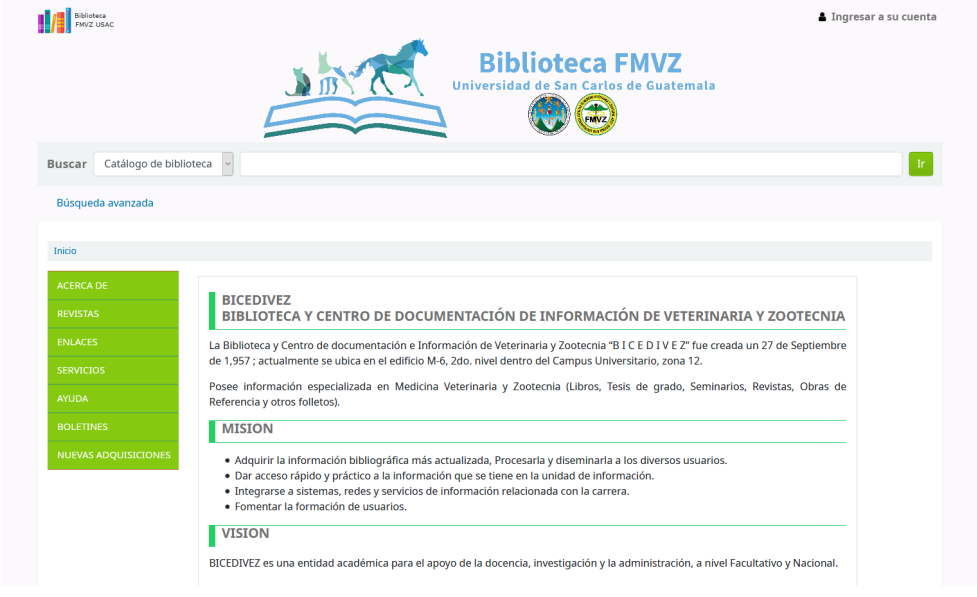
\includegraphics[width=1\linewidth]{images/05_02}
\figcaption{Página creada a través del CMS}

\end{minipage}

\end {flushleft}

\textbf{Instalación y configuración del plugin de nuevos arribos:}

Unas de las nuevas características que se instaló al sistema Koha fue el módulo de nuevos arribos, el cual es administrable por los usuarios internos de la aplicación.

Con esta nueva funcionalidad los usuarios públicos tendrán la opción de ver las últimas adquisiciones realizadas por la biblioteca.

\begin {flushleft}
\noindent\begin{minipage}[c]{\columnwidth}

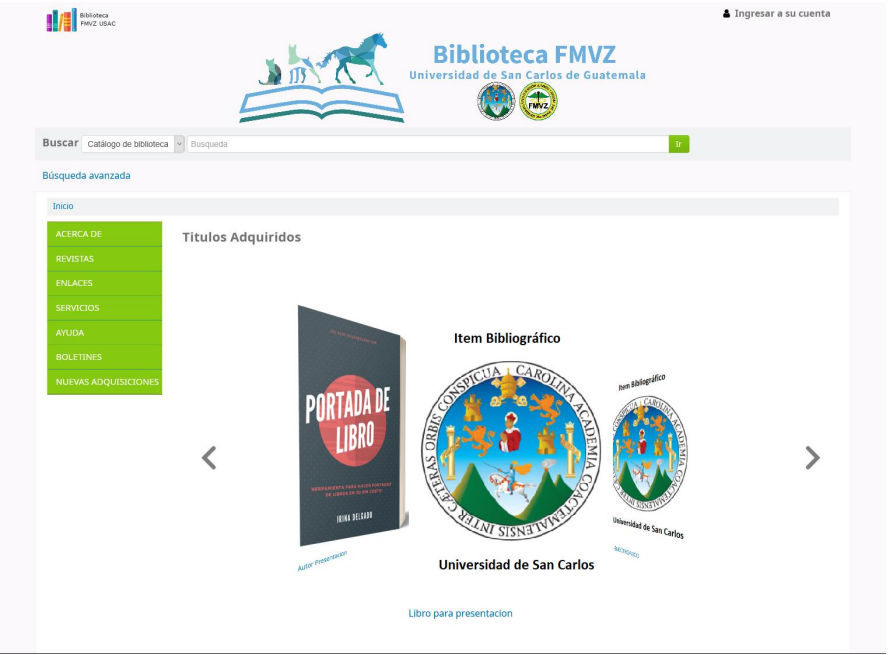
\includegraphics[width=1\linewidth]{images/05_03}
\figcaption{Página de nuevas adquisiciones}

\end{minipage}

\end {flushleft}

\textbf{Manuales:}

Se realizaron manuales para cada una de las etapas del desarrollo del proyecto, ya que existe interés por parte de otras unidades académicas en la implementación de este sistema en sus bibliotecas internas.

Además, se entregaron manuales de usuario y videos sobre el uso de los módulos de KOHA que podrán servir como medio de capacitación a nuevo personal.

\hypertarget{conclusiones-3}{%
\section{Conclusiones}\label{conclusiones-3}}

Se instaló y configuró una instancia del sistema Koha en los servidores de la Facultad de Veterinaria para la administración de la biblioteca; estos a su vez agregaron un canal de acceso al servicio de catalogación y una opción para la consulta de los elementos bibliográficos que la biblioteca posee.

La personalización de vistas del sitio público se realizó a través de creación y cambios en las hojas de estilos, además de implementar un código en JavaScript para mejorar el comportamiento y presentación del sitio. Todos estos recursos utilizados se almacenaron en una ruta dedicada a recursos estáticos, para así llevar un mejor control de cambios.

El proceso de migración de la información de la instancia antigua se realizó por medio de los módulos que Koha ofrece, realizando así un cambio transparente de la versión antigua a la más reciente que posee el sistema en mención.

\hypertarget{discusiuxf3n-de-resultados}{%
\subsection{Discusión de resultados}\label{discusiuxf3n-de-resultados}}

Los siguientes resultados fueron obtenidos realizan-
do pruebas de stress al sitio público de la biblioteca, los cuales muestran las mejoras que se obtuvieron por medio de la optimización del servidor y base de datos.

Descripción del escenario 1: para el escenario uno se efectuó una prueba ya solicitada a página principal, con una configuración de 100 usuarios, realizando una petición al servidor cada segundo.
Enlace: \url{https://bit.ly/3yZO0TK}

\begin {center}

\noindent\begin{minipage}[c]{\columnwidth}
\centering

\begin{center}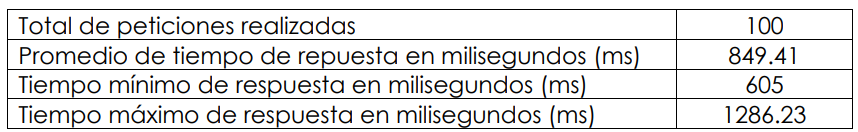
\includegraphics[width=1\linewidth]{images/05_04} \end{center}
\vspace{0.01cm}
\footnotesize
\centering

Tabla 7.1: Resultados para el escenario 1.

\end{minipage}

\end {center}

\begin {flushleft}
\noindent\begin{minipage}[c]{\columnwidth}

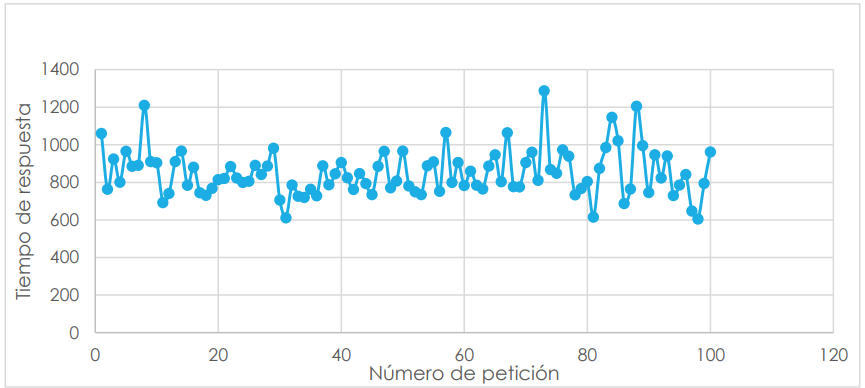
\includegraphics[width=1\linewidth]{images/05_05}
\figcaption{Tiempo de respuesta (ms) vs número de petición, escenario 1}

\end{minipage}

\end {flushleft}

Descripción del escenario 2: para el escenario dos se realizó una prueba efectuando una petición de búsqueda general, con una configuración de 100 usuarios, ejecutando una petición al servidor cada segundo.
Enlace: \url{https://bit.ly/390mH0O}

\begin {center}

\noindent\begin{minipage}[c]{\columnwidth}
\centering

\begin{center}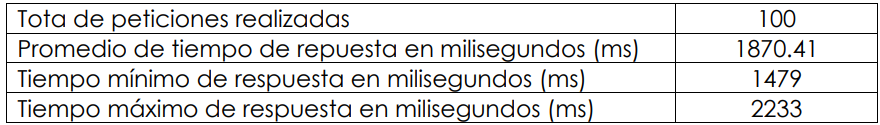
\includegraphics[width=1\linewidth]{images/05_06} \end{center}
\vspace{0.01cm}
\footnotesize
\centering

Tabla 7.2: Resultados para el escenario 2

\end{minipage}

\end {center}

\begin {flushleft}
\noindent\begin{minipage}[c]{\columnwidth}

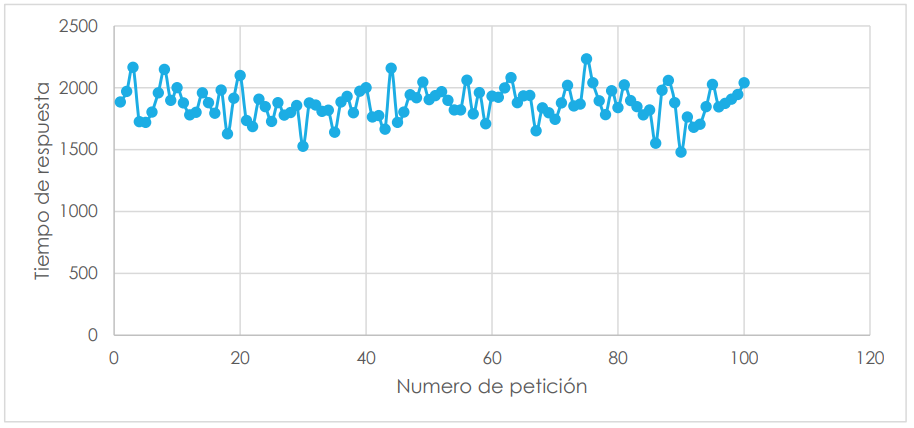
\includegraphics[width=1\linewidth]{images/05_07}
\figcaption{Tiempo de respuesta (ms) vs número de petición, escenario 2}

\end{minipage}

\end {flushleft}

Descripción del escenario 3: Para el escenario tres se realizó una prueba realizando una búsqueda avanzada, con una configuración de 100 usuarios, realizando una petición al servidor cada segundo.
Enlace: \url{https://bit.ly/3tILro8}

\begin {center}

\noindent\begin{minipage}[c]{\columnwidth}
\centering

\begin{center}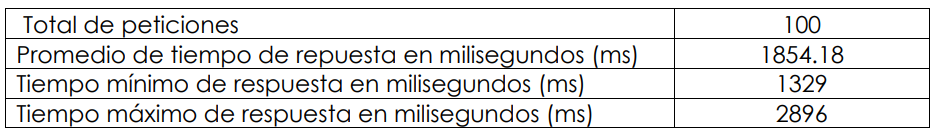
\includegraphics[width=1\linewidth]{images/05_08} \end{center}
\vspace{0.01cm}
\footnotesize
\centering

Tabla 7.3: Resultados para el escenario 3

\end{minipage}

\end {center}

\begin {flushleft}
\noindent\begin{minipage}[c]{\columnwidth}

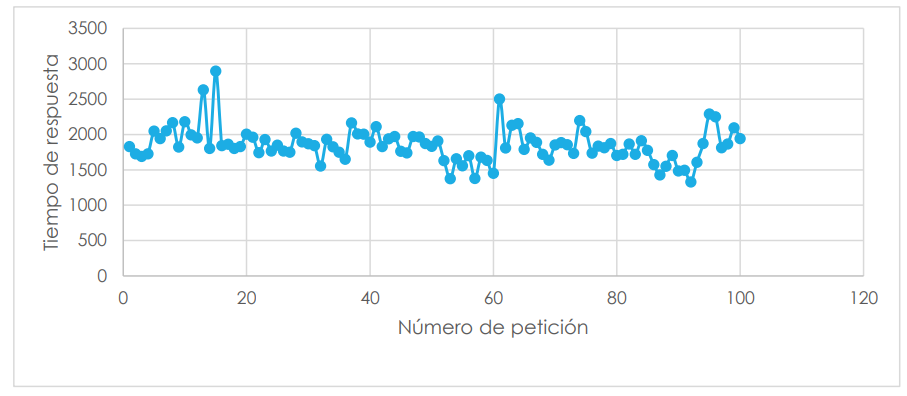
\includegraphics[width=1\linewidth]{images/05_09}
\figcaption{Tiempo de respuesta (ms) vs número de petición, escenario 3}

\end{minipage}

\end {flushleft}

Descripción del escenario 4: se realizó una prueba en conjunto, llevando a cabo un set de peticiones a la página principal, búsquedas generales y avanzadas, con una configuración de 100 usuarios para cada prueba, con un total de 300 peticiones, realizando 3 cada 3 segundos. En relación con los enlaces, se probaron todos los anteriores de forma conjunta.

\begin {center}

\noindent\begin{minipage}[c]{\columnwidth}
\centering

\begin{center}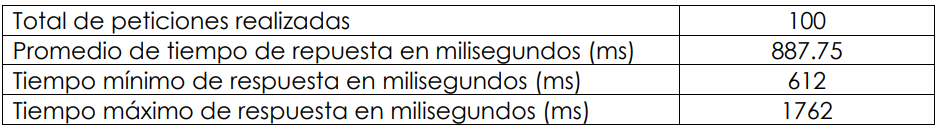
\includegraphics[width=1\linewidth]{images/05_10} \end{center}
\vspace{0.01cm}
\footnotesize
\centering

Tabla 7.4: Resultados para el escenario 4

\end{minipage}

\end {center}

\begin {flushleft}
\noindent\begin{minipage}[c]{\columnwidth}

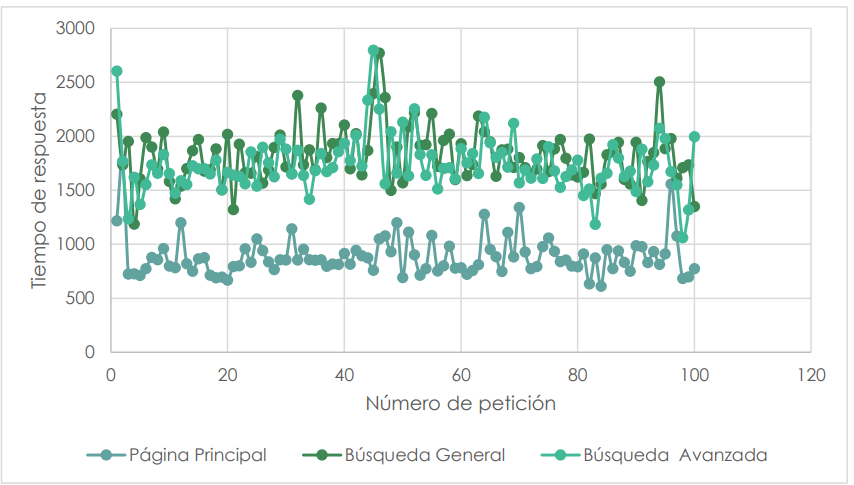
\includegraphics[width=1\linewidth]{images/05_11}
\figcaption{Tiempo de respuesta (ms) vs número de petición, escenario 4}

\end{minipage}

\end {flushleft}

Se probaron todos los enlaces de forma conjunta. Los resultados se presentan en las tablas 7.5 y 7.6.

\begin {center}

\noindent\begin{minipage}[c]{\columnwidth}
\centering

\begin{center}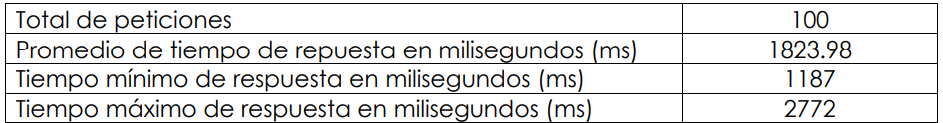
\includegraphics[width=1\linewidth]{images/05_12} \end{center}
\vspace{0.01cm}
\footnotesize
\centering

Tabla 7.5: Resultados para el escenario 5

\end{minipage}

\end {center}

\begin {center}

\noindent\begin{minipage}[c]{\columnwidth}
\centering

\begin{center}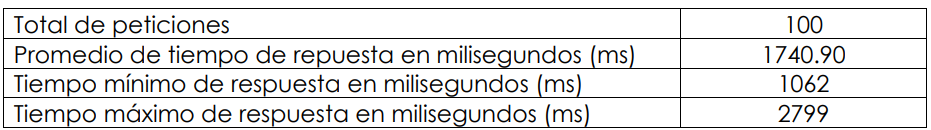
\includegraphics[width=1\linewidth]{images/05_13} \end{center}
\vspace{0.01cm}
\footnotesize
\centering

Tabla 7.6: Resultados para el escenario 6

\end{minipage}

\end {center}

\hypertarget{referencias-4}{%
\section{Referencias}\label{referencias-4}}

\begin{itemize}
\item
  {[}1{]} Gómez Vega, E. y Martín, A.), \href{https://www.ntust.edu.tw/}{«Gómez Vega, E. y Martín, A»}, \href{https://bit.ly/3z0577S}{\emph{Sistemas Integrales de gestión para bibliotecas}}, 2015. {[}En línea{]}. Disponible en: \url{https://bit.ly/2NPUSRZ}. {[}Último acceso: 01 septiembre 2020{]}.
\item
  {[}2{]} Koha, \href{https://koha-community.org/documentation/}{\emph{Documentación Oficial de Koha}}, 2021. {[}En línea{]}. Disponible en: \url{https://bit.ly/393IWDo}. {[}Último acceso: 12 agosto 2020{]}.
\item
  {[}3{]} Koha-Plugin \href{https://github.com/\%20bywatersolutions/koha-plugin-coverflow/releases/}{\emph{). Documentación oficial de Plugin de nuevos arribos}}, 2020. {[}En línea{]}. Disponible en: \url{https://bit.ly/3k3ASbO}. {[}Último acceso: 24 noviembre 2020{]}.
\end{itemize}

\end {multicols}

\medskip

\HRule

\medskip

\hypertarget{article06}{%
\chapter{Sistema de control de marcajes para los empleados del Instituto Nacional de Ciencias Forenses de Guatemala (INACIF)}\label{article06}}

\begin{center}
\includegraphics[width=1\linewidth]{images/omar} \end{center}

\begin {multicols}{2}

\hypertarget{resumen-4}{%
\section{Resumen}\label{resumen-4}}

Como parte del EPS me fue asignado el proyecto que consiste en un diseño para el control de marcaje de los empleados del Instituto Nacional de Ciencias Forenses de Guatemala (INACIF); dicho proyecto fue desarrollado utilizando diferentes tecnologías, entre ellas el uso de contenedores. La aplicación permite la administración de los biométricos con los que cuenta el instituto como la opción para generar reportes a partir de los datos que se van guardando en estos dispositivos.

\hypertarget{introducciuxf3n-6}{%
\section{Introducción}\label{introducciuxf3n-6}}

Desde el inicio de sus funciones en el año 2007, el INACIF ha buscado ser una Institución referente dentro del sector justicia de Guatemala. Como parte del fortalecimiento institucional, en el año 2010 se adquirieron dispositivos biométricos con su respectivo Software de control. Lamentablemente este se quedaba corto con las necesidades reales de la Unidad de Recursos Humanos, por lo cual se
decidió la creación de un nuevo sistema que permite el control de los marcajes de los empleados, el cual se describe en este artículo con sus características principales.

\hypertarget{artuxedculo-5}{%
\section{Artículo}\label{artuxedculo-5}}

\hypertarget{huellas-dactilares}{%
\subsection{Huellas dactilares}\label{huellas-dactilares}}

Para comprender el funcionamiento de los sistemas biométricos debe conocerse la definición de huellas dactilares. La Real Academia Española define huella dactilar como la impresión que suele dejar la yema del dedo en un objeto al tocarlo, o la que se obtiene impregnándola previamente en una materia colorante.

\hypertarget{una-breve-historia-sobre-la-biometruxeda-en-huellas-dactilares}{%
\subsection{Una breve historia sobre la biometría en huellas dactilares}\label{una-breve-historia-sobre-la-biometruxeda-en-huellas-dactilares}}

Hallazgos arqueológicos indican que las huellas dactilares se han venido utilizando para la identificación de individuos. Cabe mencionar que los más destacados son los restos de cerámica en arcilla con impresiones de huellas dactilares, que adicionalmente ayudaba a identificar el alfarero; en otras culturas como la china, presentan también sellos estampados con la huella del firmante. Sin embargo, es importante mencionar que, aunque en la época las huellas distinguían a los individuos, no existe evidencia de que estas se usaran como base universal para la identificación en ninguna de aquellas sociedades.

\hypertarget{biometruxeda}{%
\subsection{Biometría}\label{biometruxeda}}

Para abordar este tema, es importante mencionar que la biometría es usada actualmente en muchas compañías a nivel mundial, con diferentes fines como control de horarios de los empleados, acceso a diferentes sitios y más para identificación de las personas.

El concepto clásico de biometría denota la aplicación de la matemática y estadística al análisis de los datos en la ciencia biológica. Pero en el contexto tecnológico, la biometría es toda aplicación automatizada constituida por técnicas biométricas para la identificación de personas en sistemas de seguridad. Las técnicas biométricas se utilizan para clasificar las características físicas y/o de comportamiento de las personas para obtener su identidad.

\hypertarget{reconocimiento-de-huellas-dactilares}{%
\subsection{Reconocimiento de huellas dactilares}\label{reconocimiento-de-huellas-dactilares}}

Es uno de los métodos más usados en el mundo por la facilidad que tiene para apoyar los sistemas de seguridad, ya que la autenticación de personas se puede obtener de manera eficaz. La ciencia que estudia los rasgos de las huellas es la
dactiloscopia; esta se divide en cuatro grandes rasgos:

\begin{itemize}
\tightlist
\item
  Inmutabilidad: huellas que no son modificadas en el desarrollo físico de una
  persona.
\item
  Perennidad: reconoce que las personas desde los seis meses tienen huellas
  dactilares.
\item
  Variedad: huellas únicas en los individuos.
\item
  Clasificación: recopilación de información de bases de datos de aplicaciones
  con fines de control de acceso para la consulta de diferentes plantillas de
  huellas.
\end{itemize}

Los dactilogramas están compuestos por tres zonas: marginal, nuclear y bacilar. A continuación, se muestran los diferentes tipos de delta que pueden ser encontrados en las huellas dactilares.

\begin {flushleft}
\noindent\begin{minipage}[c]{\columnwidth}

\centering

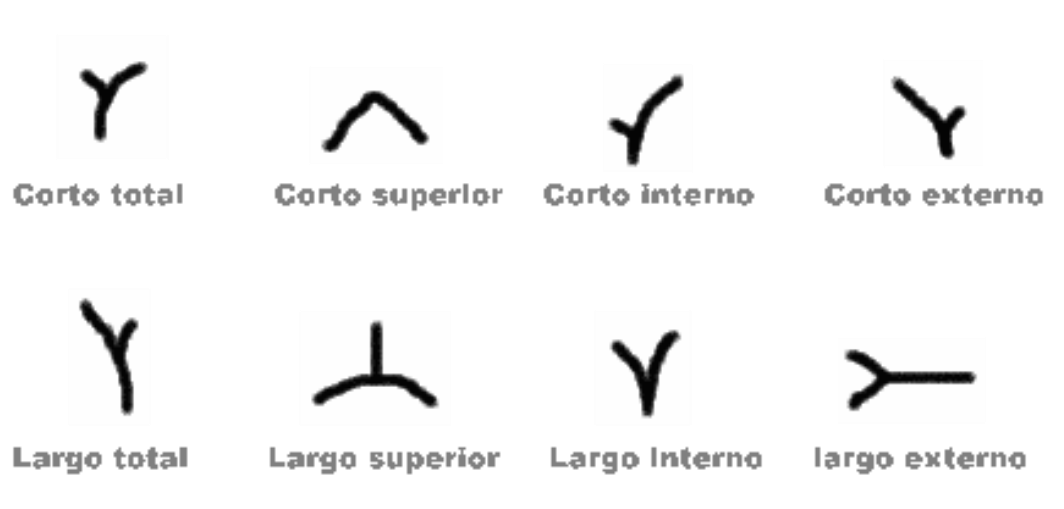
\includegraphics[width=1\linewidth]{images/06_02}
\figcaption{Deltas negros [Beavan, C (2003.) Huellas dactilares] }

\end{minipage}

\end {flushleft}

\begin {flushleft}
\noindent\begin{minipage}[c]{\columnwidth}

\centering

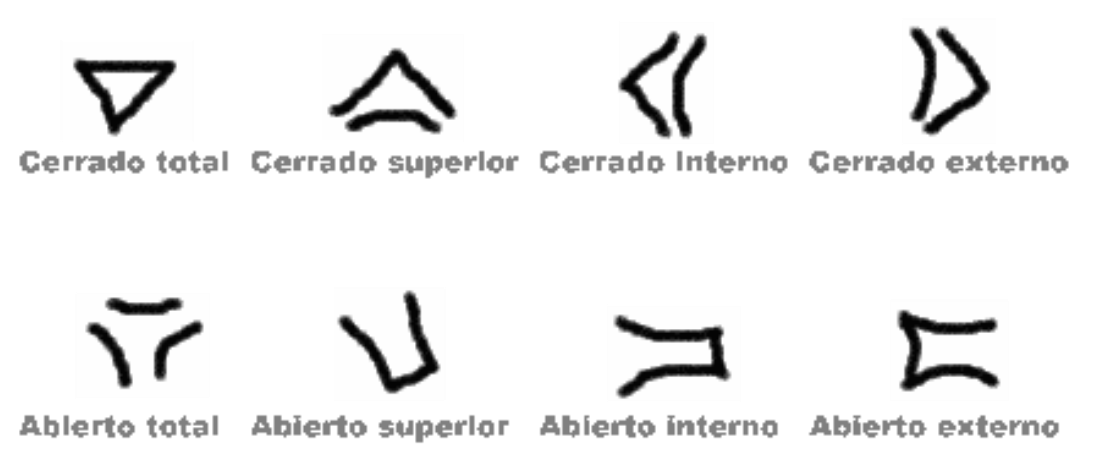
\includegraphics[width=1\linewidth]{images/06_03}
\figcaption{Deltas blancos [Beavan, C (2003.) Huellas dactilares]}

\end{minipage}

\end {flushleft}

\hypertarget{objetivos-del-proyecto}{%
\subsection{Objetivos del proyecto}\label{objetivos-del-proyecto}}

\hypertarget{objetivo-general}{%
\subsubsection{Objetivo general}\label{objetivo-general}}

Implementar una aplicación web para el control de marcajes de los empleados del Instituto Nacional de Ciencias Forenses de Guatemala (INACIF) en el departamento de Recursos Humanos.

\hypertarget{objetivos-especuxedficos}{%
\subsubsection{Objetivos específicos}\label{objetivos-especuxedficos}}

\begin{itemize}
\tightlist
\item
  Desarrollar interfaces para la integración de los lectores biométricos de huellas
  dactilares que dispone la institución, contra aplicaciones de control de acceso.
\item
  Codificar el sistema para el control de ingreso y salida mediante la
  autenticación biométrica del usuario (lector de huella dactilar).
\item
  Proveer a los usuarios correspondientes, la información condensada del historial
  de marcaje de los empleados del INACIF.
\end{itemize}

\hypertarget{descripciuxf3n-del-proyecto}{%
\subsection{Descripción del proyecto}\label{descripciuxf3n-del-proyecto}}

El proyecto consiste en implementar una herramien-
ta administrativa que permita garantizar la prestación del servicio en las diferentes dependencias del INACIF; esto por medio del registro, control y seguimiento de marcajes de los empleados de acuerdo con el rol de turnos establecidos por las diferentes áreas. Al madurar este sistema se podrán obtener indicadores de control como parte de los procesos de
evaluación del desempeño. Este sistema también alimentará a las herramientas de inteligencia de negocios y sistemas de evaluación del desempeño.

La aplicación dispone de una interfaz para realizar la conexión con los dispositivos biométricos que permiten extraer los datos que se almacenan dentro del dispositivo, para posteriormente procesar la información. También se cuenta con una aplicación web desde donde se puede administrar y manipular el sistema.

Los módulos identificados a desarrollar son los siguientes:

\begin{itemize}
\tightlist
\item
  Control de sesión
\item
  Administración de usuarios
\item
  Registro de horas
\item
  Horarios laborales
\item
  Administración de dispositivos
\item
  Configuración del software
\item
  Administración de empleados
\item
  Reportes
\item
  Ausencias
\end{itemize}

A continuación, se incluye un diagrama de contexto.

\begin {flushleft}
\noindent\begin{minipage}[c]{\columnwidth}

\centering

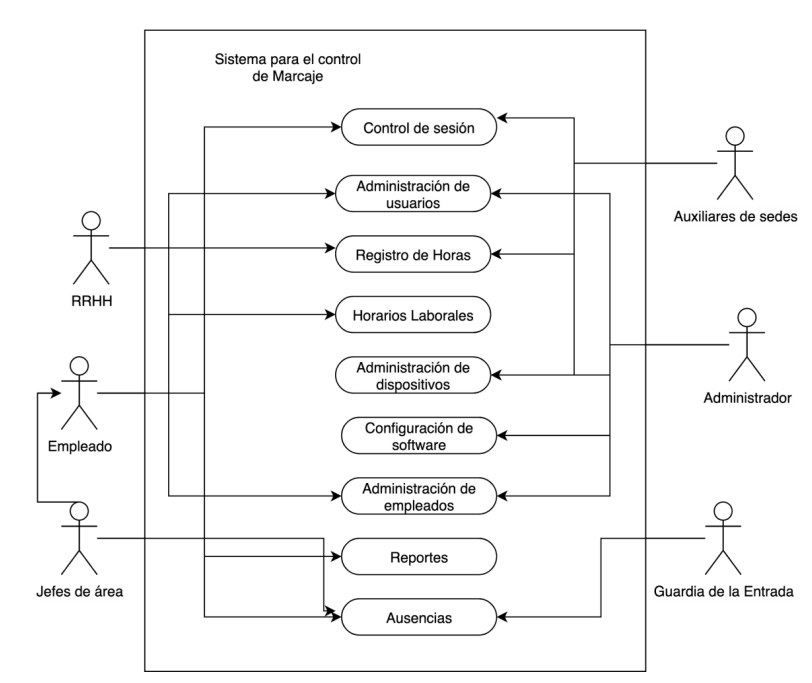
\includegraphics[width=0.7\linewidth]{images/06_04}
\figcaption{Diagrama de casos UML que muestra los módulos del sistema}

\end{minipage}

\end {flushleft}

\hypertarget{presentaciuxf3n-de-la-soluciuxf3n-del-proyecto}{%
\subsection{Presentación de la solución del proyecto}\label{presentaciuxf3n-de-la-soluciuxf3n-del-proyecto}}

El proyecto fue realizado utilizando las siguientes herramientas:

\begin{itemize}
\tightlist
\item
  Bases de datos: SQL Server
\item
  Lenguajes de programación: JavaScript y PHP
\item
  Frameworks: Vuejs y Laravel
\item
  Contenedores: Docker
\item
  Proxy: Ngnix
\end{itemize}

\hypertarget{arquitectura}{%
\subsection{Arquitectura}\label{arquitectura}}

Para el desarrollo de la aplicación se decidió utilizar contenedores para ser una solución autoescalable y de alta disponibilidad. Existen dos bases de datos, una en donde se encuentra la información del Instituto recopilada durante varios años la cual contiene datos de los empleados, sedes, puestos, números de identificación, entre otros. La otra base de datos es donde se almacena la información que se recopila de los biométricos y que utiliza la aplicación web.

\begin {flushleft}
\noindent\begin{minipage}[c]{\columnwidth}

\centering

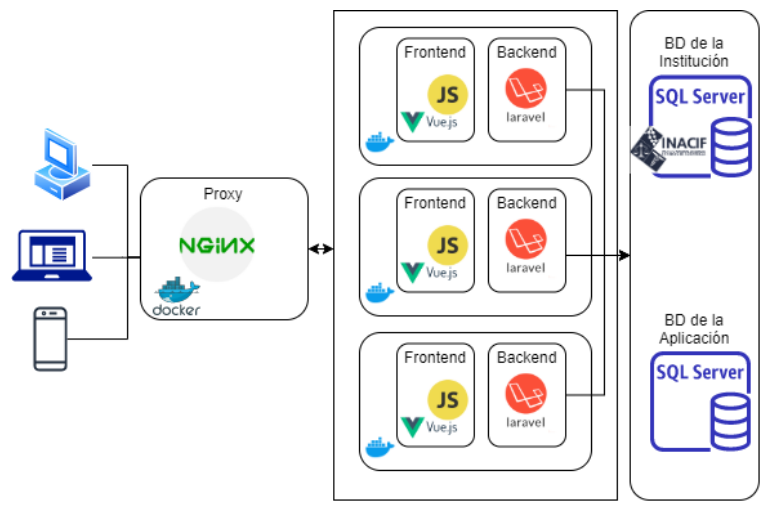
\includegraphics[width=0.8\linewidth]{images/06_05}
\figcaption{Diagrama de la arquitectura de la aplicación}

\end{minipage}

\end {flushleft}

\end {multicols}

\begin {center}
\noindent\begin{minipage}[c]{\columnwidth}
\centering

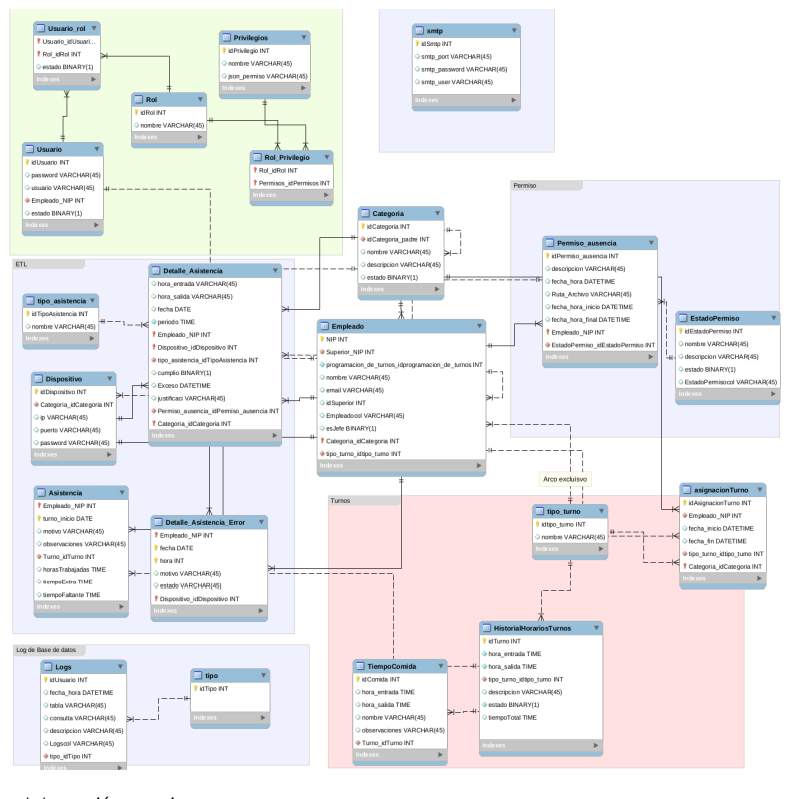
\includegraphics[width=0.5\linewidth]{images/06_06}
\figcaption{Diagrama de la base de datos}

\end{minipage}

\end {center}

\begin {multicols}{2}

\hypertarget{beneficios-del-proyecto}{%
\subsection{Beneficios del proyecto}\label{beneficios-del-proyecto}}

Al implementar un sistema informático, errónea-
mente, no se sabe transmitir su resultado algunas veces. Este, en pocas palabras, es reducir costos y llegar a ser más productivos. Además de esto se tendrá una base sólida para un crecimiento sostenible. El proyecto apoyará en diferentes áreas al Instituto Nacional de Ciencias Forenses de Guatemala.
Las áreas de mayor importancia son:

\hypertarget{uxe1rea-de-recursos-humanos}{%
\subsubsection{Área de Recursos Humanos}\label{uxe1rea-de-recursos-humanos}}

Mayor facilidad de procesamiento de datos para la generación de reportes;también centralización de información generada, traslados de datos de lostrabajadores entre las distintas sedes, cambios de horarios, asuetos por días festivos, permisos y muchas más funcionalidades.

\hypertarget{uxe1rea-administrativa}{%
\subsubsection{Área administrativa}\label{uxe1rea-administrativa}}

Se verá impactada económicamente, ya que no se tendrá un gasto en cuanto a papel, suministros y capacidad humana para dotar al área de archivo, a pesar de que se tendrá que incurrir en gastos para comprar los insumos tecnológicos y recurso humano.El área de archivo va a poder crecer (de manera electrónica) sin mayor gasto y a largo plazo el gasto será menor.

\hypertarget{empleados-del-inacif}{%
\subsubsection{Empleados del INACIF}\label{empleados-del-inacif}}

Al contar con un sistema centralizado los empleados pueden obtener reportes más certeros acerca del tiempo que pasan laborando dentro de la Institución; también ayuda a que conozcan cuál es su estado para evitar alguna llamada de atención por marcar tarde. El sistema permite generar reportes para conocer el estado de marcaje de los empleados de cualquier subsede que cuente con un dispositivo biométrico para realizar el marcaje correspondiente.

\hypertarget{costos-del-proyecto}{%
\subsubsection{Costos del proyecto}\label{costos-del-proyecto}}

La siguiente tabla muestra los costos con los que el proyecto tendría una
equivalencia directa en el mercado:

\end {multicols}

\begin {center}

\noindent\begin{minipage}[c]{\columnwidth}
\centering

\begin{center}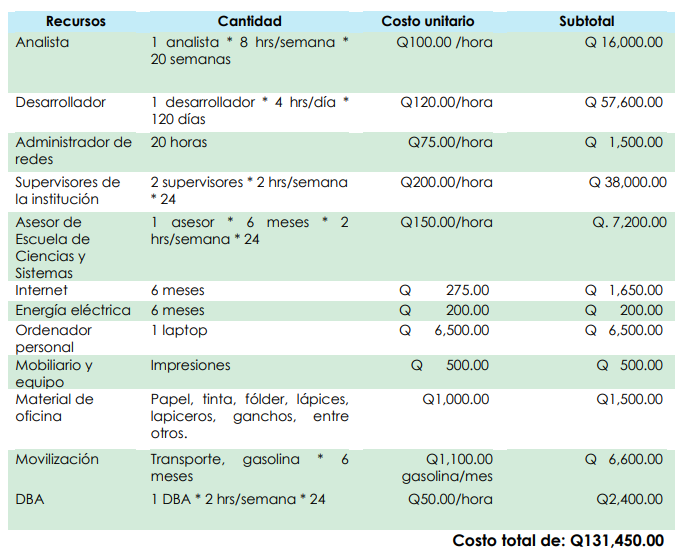
\includegraphics[width=0.5\linewidth]{images/06_07} \end{center}
\vspace{0.01cm}
\footnotesize
\centering

Tabla 8.1: Descripción de los costos del proyecto

\end{minipage}

\end {center}

\begin {multicols}{2}

\hypertarget{conclusiones-4}{%
\section{Conclusiones}\label{conclusiones-4}}

\begin{itemize}
\tightlist
\item
  Se desarrolló una interfaz que permite la comunicación entre los lectores biométricos de huellas dactilares que dispone la institución con la aplicación que se codificó.
\item
  Se codificó un sistema basado en arquitectura web que permite la gestión de marcajes de los empleados del Instituto Nacional de Ciencias Forenses de Guatemala.
\item
  Se condensó y resumió todo tipo de información para el control de marcaje, de tal manera que se puede acceder a toda esta información a través de una vista dentro del sistema.
\end{itemize}

\hypertarget{referencias-5}{%
\section{Referencias}\label{referencias-5}}

\begin{itemize}
\item
  {[}1{]} {[}«Beavan, C. Huellas dactilares.»{]}((\url{https://www.popularlibros.com/}), {[}\emph{Los orígenes de la dactiloscopia y de la ciencia
  de la identificación criminal. Editorial Alba}{]}
  (\url{https://www.popularlibros.com/libro/huellas-dactilares_178047}), 2003. {[}En línea{]}. Disponible en: \url{https://bit.ly/3hsXkcJ}. {[}Último acceso: 07 noviembre 2020{]}.
\item
  {[}2{]} \href{https://nij.ojp.gov/}{«INACIF»}, \href{https://www.inacif.gob.gt/index.php/servicios/k2-blog/item/31-la-identificacion-humana-forense}{\emph{Identificación humana forense}}, 2017. {[}En línea{]}. Disponible en: \url{https://bit.ly/3k21pGG}. {[}Último acceso: 05 febrero 2020{]}.
\item
  {[}3{]} \href{https://nij.ojp.gov/}{«Oficinas de Programas de Justicia»}, \href{https://nij.ojp.gov/library/publications/el-libro-de-referencia-de-las-huellas-dactilares}{\emph{El libro de referencia de las huellas dactilares. USA: OPJ}}, 2017. {[}En línea{]}. Disponible en: \url{https://bit.ly/3k6Ku5W}. {[}Último acceso: 17 febrero 2020{]}.
\end{itemize}

\end {multicols}

\medskip

\HRule

\medskip

\hypertarget{article07}{%
\chapter{Sistema de gestión de activos fijos para una unidad académica}\label{article07}}

\begin{center}
\includegraphics[width=1\linewidth]{images/kevin} \end{center}

\begin {multicols}{2}

\hypertarget{resumen-5}{%
\section{Resumen}\label{resumen-5}}

En el Departamento de Tesorería de la Facultad de Humanidades se llevaba a cabo el proceso de administración de los activos fijos de forma manual en su totalidad; este modo de operación consumía una cantidad exagerada de tiempo, en especial para procesos de consulta de la información; por ejemplo, la generación de solvencias para los empleados que se retiraban de la institución. En esta problemática nace la necesidad de implementar un sistema web que se encargue de la gestión de estos bienes, permita incrementar la confiabilidad de la información para las autoridades de la Facultad y a su vez se acople a la utilización de las tarjetas de responsabilidad obligatorias, según la reglamentación de la universidad. Gracias a la implementación de este sistema se optimizaron los procesos y se disminuyó el tiempo que el personal del Departamento de Tesorería invertía en los mismos, liberándolos para brindar un mejor servicio a todo el personal de la Facultad.

\hypertarget{introducciuxf3n-7}{%
\section{Introducción}\label{introducciuxf3n-7}}

El proyecto planteado se realizó con el fin de obtener la aprobación del Ejercicio Profesional Supervisado como uno de los requisitos para la graduación de Ingeniería en Ciencias y Sistemas. El proyecto consta de un sistema web que facilite el control y gestión de todos los activos fijos con los que cuenta la Facultad de Humanidades de la Universidad de San Carlos de Guatemala, debido a que el proceso se hacía de forma manual y se documentaba únicamente a través de la tarjeta de responsabilidad. Se automatizó su generación y actualización a través del sistema, lo que permite el acceso a la información de forma rápida y eficiente.

\hypertarget{artuxedculo-6}{%
\section{Artículo}\label{artuxedculo-6}}

La institución se vio en la necesidad de actualizar su proceso de gestión de los activos fijos, ya que anteriormente se realizaba de forma manual, lo que resultaba ineficiente, especialmente en el momento de requerir reportes sobre la situación actual de los bienes con los que cuenta la Facultad y al momento de generar solvencias a los empleados, ya que para hacerlo era necesario revisar las tarjetas físicamente una a una, lo que conllevaba una inversión considerable de tiempo (aproximadamente de 1 a 2 semanas); además del riesgo de errores humanos al pasar por alto alguna tarjeta. A su vez las personas a quienes se les asignaban los bienes no podían identificarse fehacientemente porque en las tarjetas no constaba el registro de personal o DPI del interesado, solamente su nombre y firma.

El sistema únicamente maneja el inventario de Activos Fijos, que se entiende como Rubro contable de propiedad, planta y equipo de una organización, lo que incluye bienes físicos destinados a ser usados en la producción o suministro de bienes y servicios para arrendarlos a terceros o para propósitos administrativos, y que se espera usar por más de un periodo (Loayza, 2006).

El registro de los bienes se realiza en una tarjeta de responsabilidad que se almacena dentro de un archivo físico; este proceso está documentado en el Manual de normas y procedimientos, específicamente en el módulo I: Registro y control de bienes muebles y otros activos fijos de la Universidad de San Carlos de Guatemala. El sistema se adhiere completamente a dicho proceso por regulación obligatoria de la universidad.

\end {multicols}

\begin {flushleft}
\noindent\begin{minipage}[c]{\columnwidth}

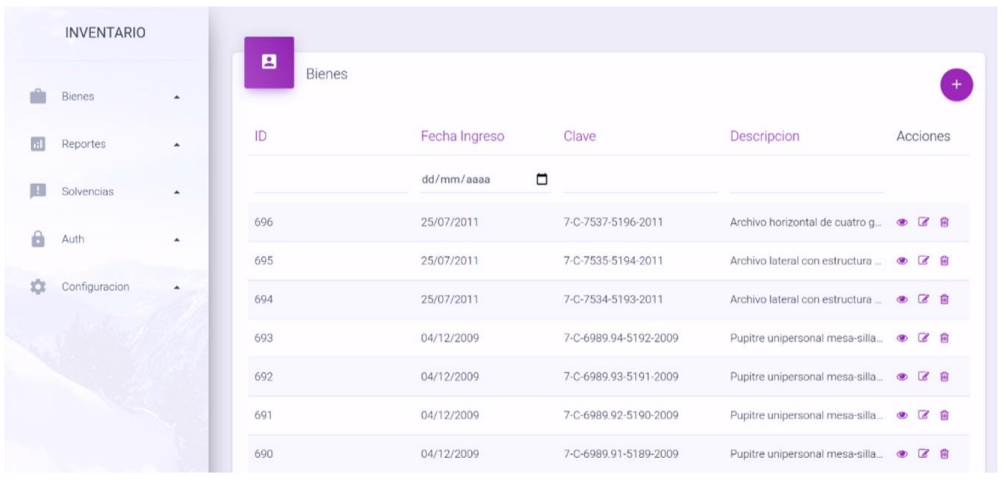
\includegraphics[width=1\linewidth]{images/07_02}
\figcaption{Pantalla de listado de bienes en el sistema de inventarios}

\end{minipage}

\end {flushleft}

\begin {multicols}{2}

La solución incluye los módulos de autenticación para gestionar el ingreso a la aplicación: un módulo de registro de bienes, reportes anuales, módulo de personal, de gestión de solvencias y de configuración.

En el módulo de registro de bienes se encuentran los ingresos, traslados y bajas de los bienes, registrando cada una de las operaciones que se realiza sobre ellos en los movimientos. Para facilitar la creación de productos se implementó un sistema de plantillas que permite definir n atributos para los productos, según su naturaleza. Por ejemplo, para un pizarrón pueden definirse atributos como ancho, alto, largo, tipo de material, entre otros. Estos atributos pueden ser usados para futuros análisis.

Se implementaron también los reportes anuales presentados por el personal encargado de inventarios, los cuales son: registro de bienes de inventarios, detalle definitivo del inventario y resumen del libro de inventarios. Estos reportes son generados con base en los movimientos de los bienes registrados en la aplicación; pueden ser generados sobre cualquier año a partir de la implementación del sistema en formato PDF para su posterior firma.

Debido a la información histórica almacenada en las tarjetas de responsabilidad y con fines de futuros análisis de comportamiento, se hace necesaria la implementación de un módulo de importación masiva donde el personal del Departamento de Tesorería pueda ingresar la información histórica al sistema a través de un archivo de MS Excel con el formato especificado. Esto incluye la validación y corrección posterior de la información ingresada. Por esta misma razón se aplican dos modos de interacción: un modo superusuario con el que puede modificarse la información sin crear registros de movimiento que tergiversen la información de los reportes y el modo normal en el cual todo cambio realizado sobre los bienes es registrado. La utilización del modo superusuario queda a discreción del Departamento de Tesorería.

El módulo de solvencias solventa el problema de generación permitiendo realizarlo de forma rápida y eficiente. Los empleados ingresarán a la plataforma desde el módulo de personal. A dicho módulo se redirecciona directamente desde la plataforma de empleados con la que ya contaba la Facultad; esta conexión está protegida mediante un token encriptado con expiración de 3 horas. Dentro del módulo de empleados pueden hacerse solicitudes de solvencias y consultar el estado de las que han sido ingresadas con anterioridad y en el de solvencias, los empleados encargados de inventarios pueden aprobar o rechazar las solicitudes, así como realizar una rápida revisión de los bienes asignados del empleado para continuar con el proceso de traslado de estos, si fuera necesario.

\begin {flushleft}
\noindent\begin{minipage}[c]{\columnwidth}

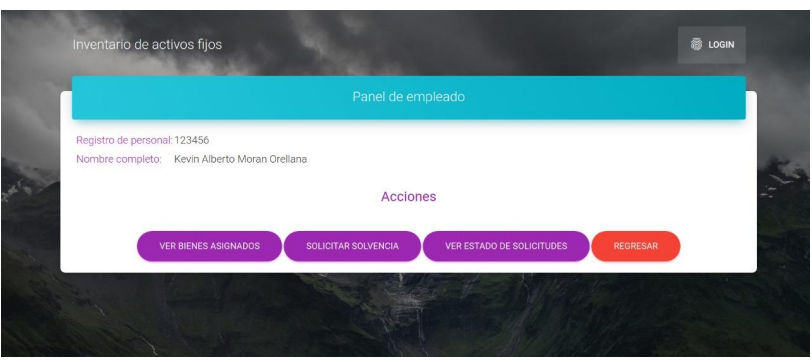
\includegraphics[width=1\linewidth]{images/07_03}
\figcaption{Pantalla de listado de solicitudes en el sistema de inventarios}

\end{minipage}

\end {flushleft}

Para gestionar la información cambiante del sistema se incluyó el módulo de configuración para gestionar los rubros, razones de movimiento y la configuración de los nombres y cargos de las personas que aparecen en los reportes anuales.

\hypertarget{conclusiones-5}{%
\section{Conclusiones}\label{conclusiones-5}}

\begin{itemize}
\item
  Se desarrolló un sistema web completo que permite el ingreso de cada uno de los activos fijos de la Facultad de Humanidades de la Universidad de San Carlos de Guatemala, así como el registro de todos sus movimientos: ingreso, traslado o baja.
\item
  Se agilizó la generación de los reportes anuales al generarlos automáticamente con base en los movimientos que son registrados por el sistema; estos reportes se pueden generar de cualquier periodo y desde el despliegue y puesta en marcha del sistema.
\item
  El diseño de la interfaz de usuario que se desarrolló facilita la comprensión del sistema y disminuye la curva de aprendizaje necesaria para poder utilizarlo.
\end{itemize}

\hypertarget{referencias-6}{%
\section{Referencias}\label{referencias-6}}

\begin{itemize}
\item
  {[}1{]} \href{https://retos-directivos.eae.es/}{«Business School, Retos directivos EAE»}, \href{https://retos-directivos.eae.es/el-activo-fijo-tipos-y-caracteristicas/}{\emph{Activo fijo: qué es, tipos, características y ejemplo }}, 2021. {[}En línea{]}. Disponible en: \url{https://bit.ly/38YnxLP} .
\item
  {[}2{]} \href{http://scielo.sld.cu/}{«Mesa, G; Serra, R. y Fleitas, S.»}, \href{http://scielo.sld.cu/scielo.php?script=sci_arttext\&pid=S2218-36202018000400154}{\emph{Metodología para la gestión de los activos fijos intangibles visibles en una universidad. Revista Universidad y Sociedad. Vol. 10, No.~4, julio a septiembre. Universidad Tecnológica de la Habana José Antonio Echeverría. Cuba}}, 2 de septiembre de 2018. {[}En línea{]}. Disponible en: \url{https://bit.ly/3supsQ6}. {[}Último acceso: 31 julio 2019{]}.
\item
  {[}3{]} \href{https://www.peoi.org/}{«Petroff, J.»}, \href{https://www.peoi.org/Courses/Coursessp/ac/fram11.html}{\emph{Activos fijos. PEOI}}, 2018. {[}En línea{]}. Disponible en: \url{https://bit.ly/2YRjuiz}. {[}Último acceso: 05 abril de 2021{]}.
\item
  {[}4{]} \href{https://kueski.com}{«StaffKueski»}, \href{https://kueski.com/blog/finanzas-personales/jovenes-emprendedores\%20/que-es-un-activo-fijo/.}{\emph{Qué es un activo fijo: definición}}, 2020. {[}En línea{]}. Disponible en: \url{https://bit.ly/3lheds6}. {[}Último acceso: 28 abril de 2021{]}.
\item
  {[}5{]} \href{https://manuales.\%20usac.edu.gt}{«Universidad de San Carlos de Guatemala»}, \href{https://manuales.usac.edu.gt/wp-content/uploads/2015/05/manualesModuloI14-07-10.pdf}{\emph{Manual de normas y procedimientos, módulo I, registro y control de bienes muebles y otros activos fijos de la Universidad de San Carlos de Guatemala. Manuales USAC}}, 2015. {[}En línea{]}. Disponible en: \url{https://bit.ly/3z0AeQR}. {[}Último acceso: 28 abril de 2021{]}.
\end{itemize}

\end {multicols}

\medskip

\HRule

\medskip

\bibliography{book.bib,packages.bib}

%%%%\printindex




\includepdf{images/contraportada.pdf}


\end{document}
